\documentclass[11pt,openright]{book}

% Reality Under Inquiry - a self-contained, editable LaTeX book project
\usepackage[utf8]{inputenc}
\usepackage[T1]{fontenc}
\usepackage{lmodern}
\usepackage{microtype}
\usepackage{xspace}
\usepackage{geometry}
\geometry{paperwidth=6in,paperheight=9in,top=0.78in,bottom=0.75in,inner=0.86in,outer=0.70in,headsep=0.22in,footskip=0.40in}
\usepackage{xcolor}
\definecolor{covernavy}{HTML}{102A43}
\definecolor{ink}{HTML}{17212B}
\definecolor{muted}{HTML}{52606D}
\definecolor{teal}{HTML}{1F7A8C}
\definecolor{pale}{HTML}{F2F6F8}
\definecolor{warm}{HTML}{FBF7F1}
\definecolor{linegray}{HTML}{D9E2EC}
\color{ink}
\usepackage{setspace}
\setstretch{1.08}
\usepackage{parskip}
\setlength{\parskip}{0.55em plus 0.15em minus 0.08em}
\setlength{\emergencystretch}{2em}
\usepackage{amsmath,amssymb,mathtools}
\usepackage{booktabs}
\usepackage{tabularx}
\usepackage{array}
\usepackage{enumitem}
\setlist{topsep=0.35em,itemsep=0.15em,parsep=0.1em}
\usepackage{tikz}
\usetikzlibrary{arrows.meta,positioning,fit,calc,shapes.geometric}
\usepackage[most]{tcolorbox}
\usepackage{titlesec}
\usepackage{fancyhdr}
\usepackage{csquotes}
\usepackage{xurl}
\usepackage{natbib}
\setcitestyle{authoryear,round,aysep={,},yysep={;}}
\usepackage{hyperref}
\hypersetup{colorlinks=true,linkcolor=teal,citecolor=teal,urlcolor=teal,plainpages=false,hypertexnames=false,pdftitle={Reality Under Inquiry},pdfauthor={Scott Brodie Forsyth}}
\usepackage{imakeidx}
\makeindex[title=Detailed Index,columns=2,intoc]

\setcounter{secnumdepth}{2}
\setcounter{tocdepth}{1}
\makeatletter
\renewcommand*{\l@section}{\@dottedtocline{1}{1.5em}{3.5em}}
\makeatother

\newcommand{\RCR}{\textsc{RCR}\xspace}
\newcommand{\LCR}{\textsc{LCR}\xspace}
\newcommand{\doop}{\operatorname{do}}
\newcommand{\E}{\mathbb{E}}
\newcommand{\Prob}{\mathbb{P}}
\newcommand{\Real}{\mathbb{R}}
\newcommand{\claim}[1]{\textbf{#1}\index{#1}}

\titleformat{\chapter}[display]
  {\normalfont\bfseries\color{covernavy}}
  {\filleft\fontsize{11}{13}\selectfont\chaptertitlename\ \thechapter}
  {0.5em}
  {\filright\fontsize{25}{29}\selectfont}
  [\vspace{0.7ex}\titlerule]
\titlespacing*{\chapter}{0pt}{-5pt}{25pt}
\titleformat{\section}
  {\normalfont\Large\bfseries\color{covernavy}}{\thesection}{0.65em}{\raggedright}
\titleformat{\subsection}
  {\normalfont\large\bfseries\color{teal}}{\thesubsection}{0.65em}{\raggedright}
\titlespacing*{\section}{0pt}{2.2ex plus .4ex minus .2ex}{0.9ex}
\titlespacing*{\subsection}{0pt}{1.6ex plus .3ex minus .2ex}{0.6ex}

\pagestyle{fancy}
\fancyhf{}
\fancyhead[LE]{\small\itshape\leftmark}
\fancyhead[RO]{\small\itshape\rightmark}
\fancyfoot[C]{\small\thepage}
\renewcommand{\headrulewidth}{0.35pt}
\renewcommand{\footrulewidth}{0pt}
\fancypagestyle{plain}{\fancyhf{}\fancyfoot[C]{\small\thepage}\renewcommand{\headrulewidth}{0pt}}
\renewcommand{\chaptermark}[1]{\markboth{\thechapter\quad #1}{}}
\renewcommand{\sectionmark}[1]{\markright{\thesection\quad #1}}

\newtcolorbox{principlebox}{
  enhanced,breakable,boxrule=0.35pt,arc=1.5pt,
  colback=pale,colframe=linegray,left=8pt,right=8pt,top=7pt,bottom=7pt,
  before skip=8pt,after skip=10pt
}
\newtcolorbox{objectionbox}{
  enhanced,breakable,boxrule=0.35pt,arc=1.5pt,
  colback=warm,colframe=linegray,left=8pt,right=8pt,top=7pt,bottom=7pt,
  before skip=8pt,after skip=10pt
}
\newtcolorbox{casebox}{
  enhanced,breakable,boxrule=0pt,arc=1.5pt,
  colback=covernavy!5,left=8pt,right=8pt,top=7pt,bottom=7pt,
  before skip=8pt,after skip=10pt
}

\newenvironment{chapterguide}{\begin{principlebox}\small\textbf{Chapter guide.}\ }{\end{principlebox}}
\newenvironment{discussion}{\begin{objectionbox}\small\textbf{Objections and discussion.}\ }{\end{objectionbox}}
\newenvironment{furtherreading}{\begin{casebox}\small\textbf{Further reading.}\ }{\end{casebox}}

\newcolumntype{Y}{>{\raggedright\arraybackslash}X}
\newcommand{\smalltable}{\small\renewcommand{\arraystretch}{1.15}}

\begin{document}

% Cover: intentionally title-only and typographically spaced.
\begin{titlepage}
  \pagecolor{covernavy}
  \color{white}
  \thispagestyle{empty}
  \vspace*{0.22\textheight}
  {\raggedright\fontsize{31}{35}\selectfont\bfseries REALITY\\UNDER INQUIRY\par}
  \vspace{1.6em}
  {\raggedright\fontsize{13}{18}\selectfont Toward an Epistemology and Ontology of Science\par}
  \vfill
  {\raggedright\large Scott Brodie Forsyth\par}
\end{titlepage}
\nopagecolor
\color{ink}

\frontmatter
\thispagestyle{empty}
\begin{center}
  {\Large\bfseries REALITY UNDER INQUIRY\par}
  \vspace{0.4em}
  {\large Toward an Epistemology and Ontology of Science\par}
  \vspace{1.2em}
  {\large Scott Brodie Forsyth\par}
\end{center}
\vfill
\noindent\rule{\textwidth}{0.35pt}\par
\small
This is an original philosophical work. Historical and scientific claims are
distinguished from interpretation, argument, and speculation. References are
given without invented quotations or page numbers; edition-specific pagination
should be checked against the copy used by a reader.
\vspace{1em}

Copyright \textcopyright\ 2026 Scott Brodie Forsyth. All rights reserved.
\clearpage

\chapter*{Abstract}
\addcontentsline{toc}{chapter}{Abstract}
Science aims at knowledge of a reality that does not depend on our wishes,
languages, or institutions. Yet scientific knowledge is produced by historically
situated people through instruments, models, measurements, statistical methods,
and social systems that can both expose and conceal the world. This book asks
whether objectivity is possible under those conditions, and if so what it means.

The answer developed here is \emph{Reflexive Constraint Realism} (\RCR). Its
ontological thesis is that a mind-independent world contains entities,
processes, and relations that constrain what can happen. Its epistemological
thesis is that claims become objective to the extent that they survive
independent routes of constraint: reliable measurement, controlled variation,
intervention, cross-context transport, model comparison, critical disagreement,
and organized attempts to find error. The account is realist without being
naive, social without being relativist, and fallibilist without treating every
belief as equally good.

\RCR distinguishes four layers of scientific success. Correspondence concerns
whether a claim is about what exists or occurs. Structural adequacy concerns
whether a representation preserves relevant relations. Interventional adequacy
concerns whether manipulating a variable changes outcomes as the model says.
Pragmatic adequacy concerns whether a representation supports reliable inquiry
and action. These layers can come apart. A model may be useful while idealized;
an entity may be real while a theory about its deeper nature is wrong; and a
prediction may succeed for the wrong causal reason. The book therefore proposes
graded ontological commitment, explicit scope conditions, and a social norm of
public corrigibility.

The framework is reconstructed through logical empiricism, falsificationism,
Kuhn, Lakatos, Feyerabend, Bayesian and error-statistical approaches, inference
to the best explanation, realism and anti-realism, pragmatism, social and
feminist epistemology, naturalized epistemology, causal inference, model-based
science, and debates about explanation, laws, reduction, emergence, values,
replication, uncertainty, and demarcation. It is then tested against cases in
physics, biology, medicine, psychology, economics, climate science, and the
social sciences. The final chapters state the theory's axioms, inferential rules,
limits, objections, and an empirical research programme.

\chapter*{Preface}
\addcontentsline{toc}{chapter}{Preface}
The philosophy of science often appears as a sequence of positions: empiricism,
falsificationism, paradigms, research programmes, Bayesianism, realism,
anti-realism, and so on. That sequence is useful, but it can give the false
impression that the central task is to choose a camp. The more demanding task is
to understand why each camp saw something important, where it overreached, and
what a coherent account of objectivity would have to preserve.

This book is written in that spirit. It does not treat science as a single
algorithm. Nor does it treat the diversity of scientific practices as evidence
that there are no standards beyond local agreement. A laboratory experiment, a
climate model, a historical dataset, a randomized medical trial, and a causal
graph do not establish claims in the same way. They can nevertheless be judged
by shared questions: What is being claimed? What would count against it? Which
parts of the result depend on instruments, models, or social assumptions? Can
the claim travel to a new setting? What would an independent critic need in
order to find an error?

The framework proposed here is original in its organization and argumentative
role, not in the sense that every component has no precedent. The literature
already contains powerful ideas about intervention, structure, mechanisms,
social criticism, error, and realism. The contribution is to place these ideas
inside one account of objective inquiry, to specify their relations, and to
make their limits explicit.

The reader will find some formal notation. It is used as a tool for precision,
not as a display of technical status. Every symbol is introduced before it is
used. Where a historical claim is compressed, the bibliography points to a
primary source or a respected scholarly treatment. Where the book advances an
interpretation, it says so. Where it speculates, it marks the speculation.

\chapter*{Introduction}
\addcontentsline{toc}{chapter}{Introduction}
Science is at once our most powerful way of learning about the world and a
human practice conducted through imperfect concepts, instruments, models,
institutions, and values. The central problem of this book is how those two
facts belong together. If science is objective, objectivity cannot mean
infallibility or a view from nowhere. If science is situated and revisable,
revisability cannot mean that evidence is powerless or that every description
is equally good.

The argument proceeds in three movements. The first reconstructs the principal
traditions in philosophy of science, from empiricism and logical positivism
through falsificationism, historical theories of change, Bayesian and
explanatory approaches, realism and anti-realism, pragmatism, and social and
feminist epistemologies. The second develops an account of observation,
models, measurement, causality, explanation, mechanisms, laws, emergence,
uncertainty, replication, and values. The third states and tests
\emph{Reflexive Constraint Realism} against cases in physics, biology,
medicine, psychology, climate science, economics, and the social sciences.

The result is a layered epistemology and ontology. It treats scientific claims
as scope-bound achievements whose warrant depends on evidence, invariance,
intervention, model transparency, and organized criticism. It also treats
their ontological force as graded: a successful pattern does not automatically
establish a hidden entity, but convergent structural and causal success can
justify increasingly strong commitments. The conclusion is a form of realism
disciplined by reflexivity, explicit uncertainty, and the possibility of
correction.

\tableofcontents

\mainmatter
\chapter{The Problem of Objectivity}
\label{ch:problem}

\begin{chapterguide}
This chapter frames the book's central problem. It distinguishes a mind-independent
world from the human practices by which claims about that world are produced.
It also introduces the four questions that any adequate philosophy of science
must answer: what exists, how evidence supports belief, what scientific
representations mean, and how institutions affect inquiry.
\end{chapterguide}

Science is successful in an ordinary and powerful sense. It predicts eclipses,
builds vaccines, identifies molecules, detects gravitational waves, estimates
the effects of policies, and changes what human beings can do. Yet success alone
does not settle what science knows. A horoscope can sometimes make a vague
prediction that appears correct. A simple model can forecast well while
misrepresenting the mechanism that generates the forecast. An institution can
produce reliable measurements while excluding the people most affected by its
research questions. Scientific success is evidence, but it is not a complete
theory of evidence.

The question of this book is therefore not whether science works. It is how
scientific work can yield objective knowledge when the work is performed by
finite, situated, interested, and fallible beings. We use concepts to identify
objects. We use instruments that embody theories. We compare observations by
statistical models. We inherit categories from institutions and languages. If
these conditions mediate every route to the world, why should the outcome be
anything more than a socially stabilized description?

The answer cannot be that scientists simply look harder. Nor can it be that
scientific claims are objective because a community accepts them. A community
can be mistaken, and a dissenting individual can be right. The answer must
explain how social practices can improve contact with a world that does not
depend on those practices.

\section{Four questions hidden inside \enquote{objectivity}}

The word \emph{objectivity}\index{objectivity} is used for several different
achievements. A measurement may be objective because different observers can
obtain it. A claim may be objective because it is not tailored to one person's
interests. A method may be objective because it makes its assumptions visible.
A theory may be objective because it tracks features of the world. These are
related but not identical.

This book separates four questions.

\begin{enumerate}[label=\textbf{\arabic*.}]
\item \textbf{The ontological question:} what, if anything, exists independently
of human observation, language, and classification? Is reality made only of
observable events, or should science also commit us to atoms, genes, fields,
social structures, or mechanisms?
\item \textbf{The epistemological question:} how can evidence justify a belief
about that reality? What is the role of observation, experiment, probability,
causal intervention, explanation, and criticism?
\item \textbf{The representational question:} what do theories and models
represent? Do they describe entities, mathematical structures, relations,
possibilities, instruments, or only the data they organize?
\item \textbf{The institutional question:} how do communities, incentives,
division of labour, expertise, funding, authority, and exclusion affect the
production of knowledge?
\end{enumerate}

A position can answer one question well and another badly. Constructive
empiricism gives a disciplined account of belief in observables while remaining
agnostic about unobservables. Structural realism identifies an important
continuity across theory change but may leave the nature of structure unclear.
Social epistemology explains why criticism by others matters but cannot by
itself guarantee that a community tracks the world. A complete account must
connect the four questions without reducing them to one another.

\section{The temptation of a single method}

The search for a single scientific method has an understandable motivation.
If there were one valid procedure, objectivity would be easy to define:
apply the procedure and accept its results. But the sciences do not have one
uniform procedure. Astronomers infer from light that cannot be manipulated in a
laboratory. Geologists reconstruct deep time from traces. Epidemiologists
compare populations under ethical constraints. Particle physicists build
detectors whose output depends on sophisticated calibration. Social scientists
study agents who respond to being studied. Mathematical scientists prove
theorems and use simulations to explore spaces too large for analytic
solutions.

This diversity does not imply that science is methodologically anarchic. It
implies that standards must be abstract enough to travel across practices
without becoming so abstract that they say nothing. The shared standard
proposed here is not a recipe but a question:

\begin{principlebox}
\textbf{Constraint question.} Which features of the claim are forced by
independent interactions with the world, and which features are supplied by the
investigator's choices of concepts, models, instruments, and purposes?
\end{principlebox}

The question can be made precise in different ways. In a randomized trial,
independence may come from treatment assignment and outcome measurement. In
climate science, it may come from the convergence of observations, physical
theory, attribution studies, and model ensembles. In a historical science, it
may come from traces that are causally connected to past events and from
independent archives. In each case the objectivity of the claim depends on the
specific constraints that resist convenient reinterpretation.

\section{Mind-independence is not observer-independence}

A reality can be independent of our concepts while being accessible only
through conceptual and technological mediation. A mountain is not created by
the word \enquote{mountain}, but the boundaries of a geological unit depend on
purposes, scale, and theory. The social category of unemployment is not a mere
illusion, but its operational definition is an institutional achievement. An
electron is not invented by a detector, but the detector's output is not
self-interpreting.

This distinction avoids two bad extremes.

\begin{itemize}
\item \textbf{Naive realism} treats perception as a transparent window and
assumes that scientific categories simply copy natural joints.
\item \textbf{Relativism} treats the dependence of descriptions on concepts as
evidence that there is no fact of the matter beyond local schemes.
\end{itemize}

The middle position requires a theory of mediation. Concepts, instruments, and
models are not obstacles that must be removed before inquiry begins. They are
means of contact. Their quality is tested by what they enable investigators to
detect, manipulate, predict, explain, and correct. A microscope does not show
\enquote{reality without mediation}. It creates a controlled relation in which
some features of a specimen become more accessible and other features become
invisible. Objectivity is achieved when the mediation is understood well enough
that the result does not depend on one unexamined viewpoint.

\section{The architecture of the argument}

The argument proceeds in three stages.

First, the major traditions are reconstructed. Logical empiricism correctly
insisted that public evidence and formal clarity matter. Popper correctly
emphasized risk and criticism. Kuhn correctly showed that research is organized
by historically situated paradigms. Lakatos correctly observed that theories are
tested as evolving programmes rather than isolated sentences. Feyerabend
correctly warned against turning a successful history into a rigid rulebook.
Bayesian epistemology correctly clarifies rational belief revision. Realist and
anti-realist traditions each identify real tensions in the relation between
successful theories and invisible entities.

Second, the practices of science are examined: measurement, model building,
explanation, intervention, mechanisms, social criticism, replication, and
uncertainty. These practices reveal that no single relation to truth is
sufficient. A good scientific representation may preserve a structure without
describing every detail. A causal claim requires more than a fitted curve. A
replication can fail because a result was false, because a population changed,
or because the original effect was context-sensitive. Institutional criticism
can increase objectivity without making evidence a product of power alone.

Third, the book develops \emph{Reflexive Constraint Realism} (\RCR), an original
framework with an ontology, an epistemology, inferential rules, and explicit
limits. The framework holds that the world is mind-independent and generative:
it produces regularities, resistances, capacities, and transformations. Science
does not mirror the whole world. It constructs representations that isolate
and track constraints relevant to a question. A claim is objective when its
support is distributed across sufficiently independent routes of inquiry and
when the inquiry exposes the conditions under which the claim would fail.

\begin{figure}[ht]
\centering
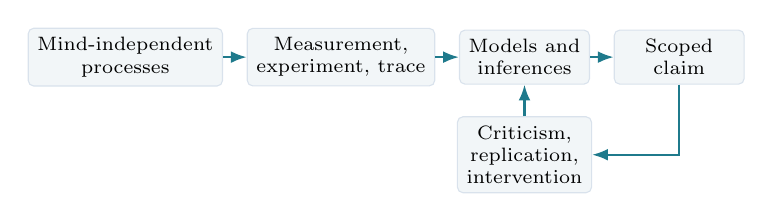
\begin{tikzpicture}[
  node distance=4mm and 3mm,
  box/.style={draw=linegray,rounded corners=2pt,fill=pale,align=center,minimum width=1.65cm,minimum height=0.68cm,font=\scriptsize},
  arrow/.style={-{Latex[length=2mm]},draw=teal,thick}
]
\node[box] (world) {Mind-independent\\processes};
\node[box,right=of world] (contact) {Measurement,\\experiment, trace};
\node[box,right=of contact] (model) {Models and\\inferences};
\node[box,right=of model] (claim) {Scoped\\claim};
\node[box,below=of model] (crit) {Criticism,\\replication,\\intervention};
\draw[arrow] (world) -- (contact);
\draw[arrow] (contact) -- (model);
\draw[arrow] (model) -- (claim);
\draw[arrow] (crit) -- (model);
\draw[arrow] (claim) |- (crit);
\end{tikzpicture}
\caption{The basic direction of \RCR: claims are grounded by contact and
tested by further constraint. The arrows are not a single linear method.}
\label{fig:rcr-cycle}
\end{figure}

\section{What would count as an answer?}

An adequate philosophy of science should not merely repeat that science is
fallible. It should specify how fallibility and objectivity coexist. It should
explain why some revisions are improvements rather than merely changes. It
should say when a model's idealization is harmless and when it distorts the
target. It should distinguish a useful forecast from a confirmed causal
mechanism. It should show how values can guide research without determining
empirical conclusions. It should explain why disagreement can be epistemically
productive in one setting and corrosive in another.

The framework developed later makes four commitments.

\begin{enumerate}
\item Reality is not constituted by inquiry, although inquiry can constitute
objects of social practice and categories of measurement.
\item Evidence is relational: its force depends on a claim, an alternative, a
measurement process, and a background model. This does not make evidence
subjective; it makes its conditions explicit.
\item Scientific representations are selective structures. Their truth is
layered rather than all-or-nothing.
\item Objectivity is a property of an inquiry system, not only of an isolated
sentence. A system is objective when it makes error discoverable by agents who
can challenge one another under transparent, world-sensitive constraints.
\end{enumerate}

These commitments are not asserted as axioms at the beginning because their
meaning depends on the history and practice that follow. The next chapters
therefore begin with the traditions that made the problem unavoidable.

\section*{Chapter summary}

The central problem is how a socially and conceptually mediated practice can
produce knowledge of a mind-independent world. Objectivity has ontological,
epistemological, representational, and institutional dimensions. Science has no
single algorithm, but its diverse methods can be evaluated by asking which
parts of a claim are constrained by independent interactions with the world.
The book's proposed answer, Reflexive Constraint Realism, treats objectivity as
stabilized world-tracking under criticism, intervention, and explicit scope
conditions.

\begin{discussion}
\begin{enumerate}
\item Is a measurement objective if all observers agree but the instrument's
calibration is unknown?
\item Can a model be scientifically valuable even if no part of it is literally
true?
\item What would count as an independent route of evidence in a historical
science where controlled intervention is impossible?
\end{enumerate}
\end{discussion}

\begin{furtherreading}
For orientation, compare the historical reconstruction in Kuhn (1962), the
realist debate in van Fraassen (1980) and Chakravartty (2007), the experimental
emphasis of Hacking (1983), and the social account of objectivity in Longino
(1990).
\end{furtherreading}

\chapter{The Empirical and Logical Traditions}
\label{ch:empiricism}

\begin{chapterguide}
Logical empiricism is reconstructed as a family of projects rather than a
single doctrine. The chapter then examines its achievements and difficulties:
the demand for public evidence, formal clarification, reduction of theoretical
claims, probability, confirmation, and the problems of meaning, holism, and
theory-ladenness. It closes with the lesson that empiricism supplies a
discipline of contact but not a complete account of objectivity.
\end{chapterguide}

The label \emph{logical positivism}\index{logical positivism} is often used as
if it named a uniform creed. Historically, the movement was more varied. The
Vienna Circle, the Berlin group, and associated philosophers disagreed about
probability, protocol statements, physicalism, conventionality, and the proper
role of metaphysics. The later label \emph{logical empiricism} is often more
accurate because several figures abandoned the strongest version of a
verification principle and developed sophisticated accounts of theoretical
terms, confirmation, and scientific language.

The broad ambition was clear: make scientific claims answerable to experience
and make their logical structure explicit. This ambition remains part of any
defensible epistemology. The problem is not the desire for evidence. The
problem is the idea that evidence can be specified without theoretical,
instrumental, historical, or social conditions.

\section{Meaning, evidence, and the rejection of pseudo-problems}

Logical empiricists sought a criterion for distinguishing statements that are
empirically meaningful from those that merely appear to make claims. A
mathematical statement could be meaningful through formal relations. An
empirical statement could be meaningful through its connection to possible
experience. Traditional metaphysical sentences were criticized when they
seemed to lack a method of verification or a clear inferential role.

The strongest charitable interpretation is methodological rather than
dismissive. The empiricists were not simply saying that everything not
immediately observable is nonsense. They were asking what difference a claim
makes to possible observation, calculation, explanation, or action. A statement
about an electron could be meaningful if it entered laws and experimental
procedures that generated testable consequences. A statement about a
transcendent entity that made no difference to any possible inquiry would not
belong to empirical science.

This motivation can be retained without adopting a strict verification
criterion. Scientific meaning is partly a matter of inferential role: what
would the claim predict, explain, license, rule out, or change in a measurement
procedure? The fact that a term is theoretical does not disqualify it. It
requires a map of how the term connects to observation and intervention.

\section{The appeal of protocol statements}

A basic problem in empiricism is the status of the observational basis.
Scientific claims are tested against observations, but observations are
reported in language and obtained under conditions. Is there a neutral layer of
protocol statements that is independent of theory?

Different empiricists proposed different answers. Some emphasized immediate
experience; others moved toward physical language, public records, or
intersubjective agreement. The movement away from private sense data was a
major strength. A scientific observation must be inspectable by others, linked
to a procedure, and embedded in a record. A private sensation can be evidence
for a person's experience, but it is not yet a public measurement.

Yet public accessibility is not the same as theoretical neutrality. To report
that a pointer moved, one needs a concept of a pointer and a rule for reading
it. To report a spectral line, one needs an instrument, a calibration procedure,
and a model connecting detector counts with wavelength. Observation sentences
are not arbitrary, but they are not self-authenticating either.

\begin{principlebox}
\textbf{Empirical contact principle.} A scientific observation is not a bare
given. It is a publicly inspectable result of a procedure that connects a
physical interaction to a claim under stated assumptions.
\end{principlebox}

This principle keeps the empiricist demand for public contact while refusing
the fantasy of an uninterpreted foundation. The later chapters will call the
stated assumptions a \emph{measurement path}: the chain from target, through
instrument and calibration, to recorded datum and interpreted result.

\section{Confirmation and the problem of induction}

Suppose a scientist observes many white swans. The observations support the
claim that all swans are white, but they do not entail it. The next swan could
be black. This is the familiar problem of induction. The problem is not
specific to swans. A theory may fit every observation collected so far and
still fail tomorrow.

Logical empiricists responded in several ways. Some treated confirmation as a
degree of support rather than proof. Reichenbach developed a probabilistic
framework in which inductive rules were justified pragmatically: if a stable
frequency existed, a suitable rule would converge toward it. Carnap attempted
to formalize degrees of confirmation. Others accepted that scientific inference
is ampliative and emphasized the practical success of prediction.

The important lesson is that evidence should change belief without pretending
to establish certainty. A rational method needs at least three ingredients:

\begin{enumerate}
\item a set of candidate claims;
\item information about how likely the evidence would be under those claims;
\item a rule for representing uncertainty and updating.
\end{enumerate}

Bayesian epistemology provides one such rule. If \(H\) is a hypothesis and
\(E\) is evidence, then Bayes' theorem is

\[
  \Prob(H\mid E)
  =
  \frac{\Prob(E\mid H)\Prob(H)}{\Prob(E)}.
\]

Here \(\Prob(H)\) is the prior probability assigned before \(E\), \(\Prob(E\mid
H)\) is the likelihood of observing \(E\) if \(H\) is true, and \(\Prob(H\mid
E)\) is the posterior probability after the evidence. The denominator
\(\Prob(E)\) makes the posterior probabilities sum to one across the relevant
alternatives.

The equation is a consistency rule, not a machine that discovers the correct
prior. If two investigators assign different priors, they may initially
disagree even after observing the same evidence. They may nevertheless converge
when the likelihood ratio is sufficiently strong. This observation will matter
later: public objectivity cannot be identified with identical starting
beliefs, but it can be strengthened by evidence that sharply discriminates
among alternatives.

\section{Theoretical terms are not optional decorations}

A strict empiricism sometimes imagines that science could be translated into
a language containing only observable predicates. But theoretical terms do
more than abbreviate observations. They organize relations among observations,
generate new questions, and make interventions possible.

Consider temperature. A thermometer reading is not identical to temperature.
The reading is produced by a physical process whose response is calibrated
against a scale. The theoretical concept of temperature links different
instruments, equilibrium conditions, equations, and predictions. Removing the
term would not make the science more empirical; it would make the connections
harder to express.

The same point applies to genes, fields, utility, inflation expectations, and
neural representations. Some of these terms refer to entities, some to
properties, some to model variables, and some to institutional constructs.
They should not all receive the same ontological status. But they cannot be
evaluated merely by asking whether they are directly observed.

A scientific term earns epistemic standing by the role it plays in a network
of constraints. It should connect to measurement, support counterfactuals,
survive alternative operationalizations, or make possible reliable
intervention. The term becomes suspicious when it is insulated from every
possible correction and is used only to redescribe its own successes.

\section{Holism and the Duhem--Quine problem}

An isolated hypothesis rarely entails an observation by itself. A prediction
typically depends on auxiliary assumptions about initial conditions,
instruments, background laws, numerical approximations, and data processing.
When the prediction fails, several components may be responsible. This is the
problem associated with Duhem and later Quine.

Quine's critique of the analytic--synthetic distinction extended the point:
beliefs form a web, and experience bears on the web as a whole rather than on
single statements one at a time \citep{duhem1906,quine1951}. The strongest
lesson is epistemic humility. A failed prediction does not automatically
identify which sentence is false.

The bad lesson would be that no claim can be tested. Scientific practice
responds by designing tests that vary or stabilize different parts of the
network. Independent instruments can challenge calibration assumptions.
Different initial conditions can test a law across regimes. Replication teams
can use the same data with alternative pipelines. Interventions can isolate
causal components. A theory can therefore be tested holistically, but not
indiscriminately.

\begin{table}[ht]
\centering
\smalltable
\begin{tabularx}{\textwidth}{p{0.29\textwidth}YY}
\toprule
Empiricist insight & What it protects & What it cannot by itself supply\\
\midrule
Public evidence & Shared access and correction & A theory-neutral observation language\\
Formal clarity & Explicit inferential commitments & A choice of relevant variables\\
Probability & Graded belief and uncertainty & A unique prior or causal interpretation\\
Operational connection & Contact between concepts and procedures & A guarantee that the operation measures the intended target\\
\bottomrule
\end{tabularx}
\caption{What the logical empiricist tradition contributes, and where it needs
supplementation.}
\label{tab:empiricist-lessons}
\end{table}

\section{What survives}

The logical empiricist tradition contributes four durable norms.

First, scientific claims should be connected to public procedures. A claim that
cannot alter any observation, intervention, or inferential practice is not a
scientific claim merely because it uses technical words.

Second, the relation between theory and evidence should be made explicit.
Scientists should state what assumptions a result depends on and what would
change if those assumptions were relaxed.

Third, uncertainty should be represented rather than hidden behind categorical
language. A point estimate without an error model can be less informative than
a range with clear limitations.

Fourth, philosophical arguments benefit from formal reconstruction. Logic and
probability do not replace empirical inquiry, but they expose ambiguities and
show exactly where an inference requires an extra premise.

What does not survive is the idea of a purely given foundation, a universal
translation into observation language, or an automatic rule for induction.
Objectivity will require a broader account of constraints: experimental,
statistical, causal, historical, and social.

\section*{Chapter summary}

Logical empiricism is best understood as a diverse attempt to connect meaning
and justification to public evidence and logical structure. Its strongest
achievements are the demand for inspectable procedures, explicit inferential
commitments, probabilistic uncertainty, and clarity about theoretical terms.
Its weaknesses arise when observation is treated as theory-neutral or when
confirmation is expected to yield certainty. Holism shows that tests involve
networks of assumptions, but independent instruments, interventions, and
replications can still distribute and localize criticism.

\begin{discussion}
\begin{enumerate}
\item Does a claim become scientific when it has a possible observation, or
does it also need a reliable measurement path?
\item Should a theoretical entity be accepted if it improves prediction but
does not support intervention?
\item How should two investigators with different priors resolve a disagreement?
\end{enumerate}
\end{discussion}

\begin{furtherreading}
Read Reichenbach (1938) for a mature probabilistic empiricism, Hempel (1965)
for the logic of explanation, Quine (1951) for holism, and the historical
overview of logical empiricism in the relevant essays collected by Carnap and
his contemporaries.
\end{furtherreading}


\chapter{Falsification, Revolutions, and Research Programmes}
\label{ch:change}

\begin{chapterguide}
This chapter moves from the logic of evidence to the history of scientific
change. Popper's falsificationism, Kuhn's account of normal and revolutionary
science, Lakatos's research programmes, and Feyerabend's methodological
pluralism are treated as complementary diagnoses of different pressures within
science. The central question is whether historical change destroys rational
progress or reveals a more complex form of it.
\end{chapterguide}

The logical empiricist image of science was often read as a picture of
hypotheses confronting observations one by one. Karl Popper objected that this
picture misunderstands the asymmetry between confirmation and criticism.
Universal statements cannot be conclusively verified by finite observations,
but a universal statement can conflict with a particular observation once the
auxiliary conditions are fixed. Popper therefore emphasized conjectures,
deductive consequences, and attempts at refutation \citep{popper1959}.

Later historians and philosophers showed that scientific practice does not fit a
simple rule of immediate abandonment. Anomalies are common. Instruments fail.
A theory may be central to a research programme and worth preserving while an
auxiliary assumption is revised. Scientific communities work within inherited
standards and problem-solutions. The important task is not to choose between
logic and history but to understand how criticism operates inside historical
practice.

\section{Popper's strongest falsificationism}

Popper's positive thesis is not that scientists can mechanically prove theories
false. A scientific theory is exposed to risk when it rules out possible
observations and when its predictions are precise enough to be vulnerable. A
theory that accommodates every possible outcome by changing its interpretation
after the fact is not thereby scientific.

This is a criterion of \emph{testability}, not a complete description of
scientific careers. It explains why a bold theory can be epistemically
valuable even before it is established: it tells us what the world would have
to be like for the theory to fail. It also explains why ad hoc adjustments are
suspicious when they merely protect a claim from evidence without generating
new constraints.

Popper's account remains useful for demarcation and scientific honesty. It is
not enough to collect confirming examples. A serious claim should expose
itself to possible failure. But two qualifications are necessary.

First, observations do not test isolated theories. A failed prediction can
reflect an instrument error, a hidden confounder, or a mistaken initial
condition. Second, a theory may rationally survive an anomaly when it is part
of a productive programme whose other consequences are successful. Immediate
falsification is too crude as a rule of practice.

\section{Kuhn and the structure of scientific change}

Thomas Kuhn's account of scientific revolutions begins with a historical
observation: much of mature science is not a continuous search for decisive
tests of foundational principles. Scientists work within a paradigm, solving
puzzles using shared exemplars, standards, instruments, and concepts
\citep{kuhn1962}. This normal science is conservative in a productive sense.
It concentrates effort and permits detailed work that would be impossible if
every assumption were reopened at every moment.

A paradigm can nevertheless generate persistent anomalies. When the anomalies
interact with practical failures, new instruments, or a rival conceptual
framework, a period of crisis may arise. A revolution changes not only an
isolated theory but the questions that count as important, the objects that
are salient, and the standards by which solutions are judged.

The strongest reading of Kuhn is not that scientists live in private worlds
with no contact across paradigms. Kuhn explicitly retained a notion of
progress in puzzle-solving and argued that later theories often extend the
range and precision of problems that can be addressed. His discussion of
incommensurability concerns difficulties of translation and comparison, not a
claim that all theories are equally good.

Kuhn's insight is that standards are partly embodied in practice. A criterion
such as simplicity or accuracy does not decide theory choice without a
background understanding of what counts as a relevant problem and a workable
representation. The danger is that this insight can slide into relativism if
the shared world disappears from the account. Anomalies are not merely
failures to fit a community's expectations; they can be persistent effects
generated by the world.

\section{Lakatos and the time-scale of criticism}

Imre Lakatos attempted to retain Popperian rationality while acknowledging the
historical endurance of research traditions. A research programme has a
\enquote{hard core} of central commitments, a \enquote{protective belt} of
auxiliary hypotheses, and heuristic rules guiding the development of the
programme \citep{lakatos1970,lakatos1978}. Scientists do not abandon a
programme after every anomaly. They compare programmes over time.

A programme is progressive when modifications produce new empirical content
and some of that content is corroborated. It is degenerating when changes
primarily accommodate known facts without leading to novel success. The
standard is comparative and historical. A theory is not condemned by a single
bad result, but a programme can lose rational support if a rival repeatedly
generates and confirms more demanding results.

Lakatos improves both Popper and Kuhn. He captures the importance of research
continuity without treating persistence as irrational, and he turns the vague
idea of paradigm success into a comparative methodological question. But the
criterion is not mechanically decisive. The distinction between a novel
prediction and a post hoc accommodation can depend on how a research history
is reconstructed. A degenerating programme can recover after a long pause.
Science also contains multiple programmes that address different targets and
cannot be ranked on a single scale.

\section{Feyerabend and the criticism of methodological monism}

Paul Feyerabend argued that no fixed methodological rule captures the history
of major scientific advances. The case of Galileo, for example, involved
conceptual, instrumental, rhetorical, and experimental strategies that would
look illegitimate if judged by a narrow rule of confirmation. Feyerabend's
provocation was directed not only at method but at the political authority that
can arise when one method is treated as a monopoly \citep{feyerabend1975}.

The charitable interpretation is pluralist rather than nihilist. Scientific
progress can require changing the standards by which a problem is approached.
Alternative theories can reveal the hidden assumptions of a dominant theory.
A period of methodological diversity may be epistemically useful because it
prevents a community from becoming blind to its own categories.

The strongest objection to Feyerabend is that \enquote{anything goes} cannot
itself be a sufficient norm. Some practices are more transparent, more
reliable, and more capable of correcting error than others. A community that
suppresses criticism or protects a claim from every possible test is not
rescued by historical pluralism. \RCR\ accepts methodological diversity but
asks what constraints the method creates and whether those constraints are
genuinely world-sensitive.

\section{Are revolutions rational?}

The phrase \enquote{scientific revolution} can suggest a discontinuity so
complete that rational comparison becomes impossible. There is a real issue
here: concepts change their meaning when their inferential role changes. The
term \enquote{mass} in Newtonian mechanics is not simply the same term as
relativistic mass. Some standards shift with the problem situation.

Yet complete discontinuity is too strong. A later theory may preserve limiting
relations, numerical results, experimental techniques, or causal interventions
from an earlier one. Old concepts may survive as approximations within a
restricted domain. Even when vocabularies change, laboratories, bodies,
detectors, and failed predictions can constrain both sides.

\begin{principlebox}
\textbf{Historical continuity principle.} Rational comparison across theories
does not require a vocabulary-free standpoint. It requires enough shared
constraints that rival representations can be linked to common phenomena,
operations, or consequences, even when their concepts are not fully
intertranslatable.
\end{principlebox}

This principle also clarifies why scientific progress is not mere accumulation.
A later theory can improve a representation by changing the dimensions along
which the phenomenon is understood. Progress may be conceptual, predictive,
causal, experimental, or organizational. It is not a single scalar quantity.

\section{The lesson for objectivity}

These traditions yield a layered picture of scientific rationality.

\begin{table}[ht]
\centering
\smalltable
\begin{tabularx}{\textwidth}{p{0.22\textwidth}YY}
\toprule
Tradition & Key achievement & Required correction\\
\midrule
Popper & Risk, criticism, testability & Tests involve auxiliary assumptions and time\\
Kuhn & Practice, paradigms, conceptual change & Revolutions remain constrained by shared phenomena\\
Lakatos & Comparative research programmes & Progress is plural and historically underdetermined\\
Feyerabend & Methodological pluralism and criticism of monopoly & Pluralism needs standards of transparency and error correction\\
\bottomrule
\end{tabularx}
\caption{Four accounts of scientific change and the constraints needed to
make them compatible.}
\label{tab:change-traditions}
\end{table}

Scientific objectivity cannot be identified with resistance to all change. A
dogmatic theory can survive anomalies. Nor can it be identified with change
itself. A community can shift because of fashion, power, or institutional
pressure. Objectivity concerns the quality of the constraints that govern
change: whether anomalies are investigated, alternatives are developed,
evidence is independently checked, and revisions increase the range and
reliability of world-directed inference.

\section*{Chapter summary}

Popper shows why risky claims and attempts at refutation matter. Kuhn shows
that scientists work within paradigms and that revolutions change problems and
standards. Lakatos explains why rational criticism often operates over the
history of research programmes rather than through instant rejection.
Feyerabend warns against methodological monopoly and reminds us that new
methods can be necessary for new problems. Together they support a fallibilist,
historical, and plural account of rationality, provided that theory change
remains constrained by common phenomena, interventions, and error correction.

\begin{discussion}
\begin{enumerate}
\item When should an anomaly be treated as evidence against a theory rather
than as a reason to revise an auxiliary assumption?
\item Can a research programme be progressive in one domain and degenerating in
another?
\item Does conceptual incommensurability prevent rational comparison, or only
make comparison more demanding?
\end{enumerate}
\end{discussion}

\begin{furtherreading}
Compare Popper (1959), Kuhn (1962), Lakatos (1970), and Feyerabend (1975)
directly. For critical discussion of historicist rationality, consult the
relevant scholarship on scientific change and the essays collected in
Lakatos and Musgrave (1970).
\end{furtherreading}


\chapter{Realism, Anti-Realism, and the Problem of Success}
\label{ch:realism}

\begin{chapterguide}
This chapter asks what the success of science licenses us to believe. It
examines constructive empiricism, scientific realism, structural realism,
entity realism, pragmatism, inference to the best explanation, and the
pessimistic meta-induction. The chapter's conclusion is a layered conception of
truth and a graded account of ontological commitment.
\end{chapterguide}

The central realist argument is simple. Mature scientific theories often
predict novel phenomena, integrate diverse observations, guide new instruments,
and support interventions. It would be a remarkable coincidence if the
theoretical entities and structures responsible for this success were entirely
fictional. Scientific realism therefore recommends belief in at least some
unobservable aspects of the world described by our best theories
\citep{chakravartty2007}.

The anti-realist replies that success need not reveal truth. A theory can be
empirically adequate: it can correctly describe what is observable while
remaining agnostic about unobservable entities. Bas van Fraassen's constructive
empiricism is not a claim that electrons do not exist. It is a claim about the
epistemic attitude required by science: acceptance may involve belief that a
theory is empirically adequate without belief that its unobservable posits are
true \citep{vanfraassen1980}.

Both positions contain an important distinction. The question is not whether a
scientist may use a model containing unobservables. Scientists plainly do.
The question is what attitude the use and success of the model rationally
warrant.

\section{Constructive empiricism}

Constructive empiricism avoids a crude instrumentalism. It can accept that
scientific theories are true-or-false claims, that they explain phenomena, and
that scientists can rationally adopt them for practical purposes. Its
distinctive requirement is epistemic modesty: belief need extend only to
observable adequacy.

This view has several strengths. It respects the historical fact that
successful theories are often replaced. It avoids treating every useful
mathematical posit as an entity. It separates the aim of science from the
psychology of individual scientists. And it recognizes that seeing through a
microscope or detector involves a complex notion of observability rather than
an absolute line between the visible and invisible.

Its difficulty is that the observable/unobservable distinction can be unstable
and method-dependent. A virus, a distant galaxy, and a magnetic field do not
form a natural epistemic class. More importantly, empirical adequacy can be
achieved by models whose internal structure supports counterfactual and
interventional reasoning. If a theory's unobservable components are repeatedly
used to make new kinds of contact with the world, permanent agnosticism may be
too restrictive.

\section{Scientific realism and the no-miracles intuition}

Realists often appeal to the no-miracles argument: the ability of science to
predict and intervene would be extraordinary if theories were not at least
approximately true. The argument is not a deductive proof. It is an inference
to the best explanation (IBE)\index{inference to the best explanation}. We
compare explanations of scientific success and regard truth-tracking as one
candidate.

Gilbert Harman used the phrase \enquote{inference to the best explanation} for
the pattern in which a hypothesis is selected because it would, if true,
explain the evidence better than alternatives \citep{harman1965}. IBE is not a
license to accept whatever story feels satisfying. A good explanatory
hypothesis should have independently supported consequences, expose itself to
failure, and outperform rivals in a specified domain.

The no-miracles argument is strongest when success is robust across
independent routes: a theory predicts an effect before it is observed, survives
instrumental changes, connects different phenomena, and supports interventions
that would not be possible if the relevant structure were absent. It is weaker
when the success is merely a fit to existing data, depends on flexible
parameters, or is achieved by many unrelated models.

\section{The pessimistic meta-induction}

The historical record supplies an obvious challenge. Many past theories were
successful and yet contained entities or principles that later scientists
rejected. The luminiferous ether supported a useful wave theory of light.
Phlogiston organized chemical phenomena before oxygen chemistry. Classical
mechanics remains reliable in many domains although its ontology is not the
final physical description.

The pessimistic meta-induction argues that our current theories may be like
those past theories: successful for a time but false in their unobservable
commitments. This is not a proof of anti-realism. It is a warning against
treating present success as a guarantee of total truth.

The realist response often distinguishes between abandoned structures and
retained structures. A later theory may reject an entity while preserving
equations, symmetry relations, limiting cases, or causal dependencies. John
Worrall's structural realism emphasizes precisely this possibility
\citep{worrall1989}. The theory changes, but some relations survive.

The response is plausible but incomplete. Mathematical structure is not a
single object. One must specify which structure is retained, at what level, and
under what transformations. A merely formal similarity can survive while the
physical interpretation changes. \RCR\ therefore treats structural continuity
as evidence, not as an automatic guarantee of truth.

\section{Structural realism}

Structural realism comes in epistemic and ontic forms. Epistemic structural
realism says that science gives us knowledge of relations or structure even if
knowledge of the intrinsic nature of entities remains limited. Ontic structural
realism makes the stronger metaphysical claim that structure is more
fundamental than objects.

The epistemic version fits an important pattern in theory change. A relation
such as a mathematical dependency may survive when the entities used to
interpret it change. The relational pattern can therefore be a better target of
realist commitment than the full ontology of a theory.

The ontic version is more ambitious but faces questions about what a structure
is without relata, how structures are individuated, and how causal powers fit
into a purely relational picture. \RCR\ remains neutral between object-first
and structure-first metaphysics at the ultimate level. It claims only that
scientific evidence often supports structured constraints more securely than
an exhaustive inventory of intrinsic natures.

\section{Entity realism and intervention}

Ian Hacking shifted attention from representation to intervention. When
scientists can use an entity to create stable effects in other systems, there
is a strong practical reason to believe that the entity is not merely a
calculational fiction \citep{hacking1983}. This is especially persuasive in
experimental settings where the entity is not just inferred from the same data
that the theory was designed to fit.

Intervention is not infallible. A successful manipulation can be described by
different ontologies. An instrument may be responding to a field, a mechanism,
or a composite process. Experimental control can also be achieved through a
model whose components are only approximately isolated.

The lesson is therefore conditional. Intervention raises the ontological
status of a posit when the effect is robust under changes in apparatus,
calibration, and background assumptions, and when the posit makes a difference
to outcomes that were not used to define it. This will become one of the
criteria in \RCR's commitment ladder.

\section{Pragmatism without relativism}

Pragmatist traditions, especially Peirce's account of inquiry, emphasize that
belief is a habit of action and that the meaning of an idea lies partly in its
conceivable practical consequences \citep{peirce1878}. This is not the claim
that truth means whatever works for a person. Peirce's ideal of inquiry is
public, fallible, and oriented toward a community that could continue testing
the claim.

Pragmatism corrects two realist errors. First, it reminds us that theories are
tools for asking questions and changing situations, not museum labels attached
to a finished world. Second, it prevents the search for truth from becoming
detached from the practices that give concepts their use.

It also needs correction. Immediate usefulness can reward a false model,
especially when a short-term prediction is obtained through a fragile
correlation. \RCR\ distinguishes pragmatic adequacy from correspondence and
causal adequacy. A model can be useful while its ontological interpretation
remains uncertain.

\section{A layered account of truth}

The debate becomes less confusing when different kinds of scientific success
are separated.

\begin{table}[ht]
\centering
\smalltable
\begin{tabularx}{\textwidth}{p{0.22\textwidth}Y Y}
\toprule
Layer & Question & Typical evidence\\
\midrule
Correspondence & Does the claim identify what exists or occurs? & Independent detection, historical trace, convergent measurement\\
Structural accuracy & Does the representation preserve relevant relations? & Invariance, limiting cases, cross-domain integration\\
Interventional adequacy & Does changing the represented variable change outcomes as expected? & Experiment, manipulation, mechanism, counterfactual test\\
Pragmatic adequacy & Does the representation support reliable inquiry or action? & Forecasting, control, diagnosis, design\\
\bottomrule
\end{tabularx}
\caption{Four layers of scientific success. They support one another but do not
collapse into one another.}
\label{tab:truth-layers}
\end{table}

A model may be structurally accurate in a restricted regime while being
literally false outside it. A variable may be useful for intervention without
being a fundamental entity. A theory may correspond to a real mechanism while
its mathematical idealization misstates the mechanism's fine detail. The
proper question is not whether the whole theory is simply true, but which
claims, structures, and interventions have earned which kinds of commitment.

\begin{principlebox}
\textbf{Layered truth principle.} Scientific truth is not one undifferentiated
property. A claim may be correct about a phenomenon, structurally correct
about a relation, causally adequate for an intervention, and pragmatically
useful to different degrees. Objectivity improves when these layers are
reported separately rather than compressed into one label.
\end{principlebox}

\section{What realism should commit us to}

\RCR\ rejects both the demand for literal truth of every model component and
the refusal to believe in any unobservable. It recommends graded commitment.

\begin{enumerate}
\item Believe an observable event when its measurement path is reliable and
alternative explanations have been tested.
\item Treat a structure as objectively supported when it remains stable across
independent representations and transformations.
\item Treat an entity or mechanism as strongly supported when intervention,
convergence, and counterfactual robustness all point to it.
\item Treat a theoretical ontology as provisional when its success is confined
to prediction or depends on highly flexible idealization.
\end{enumerate}

This is not an attempt to turn realism into a numerical score. It is a
discipline of separating what the evidence supports from what the imagination
adds. The final commitment should be proportional to the strongest constraint
that the inquiry has actually established.

\section*{Chapter summary}

Constructive empiricism protects epistemic modesty; scientific realism explains
why robust success can support belief in unobservables; structural realism
highlights continuity of relations; entity realism emphasizes intervention; and
pragmatism links meaning to public inquiry and action. The pessimistic
meta-induction warns that successful theories can contain false commitments.
The proposed response is layered truth and graded commitment: correspondence,
structural, interventional, and pragmatic adequacy are distinct dimensions of
scientific success.

\begin{discussion}
\begin{enumerate}
\item Is an entity more credible when it can be manipulated, or can
intervention itself be theory-dependent?
\item Which parts of a modern scientific theory seem most secure: entities,
equations, structures, mechanisms, or measurement procedures?
\item Can empirical adequacy be enough for practical science even when
ontology is unsettled?
\end{enumerate}
\end{discussion}

\begin{furtherreading}
Read van Fraassen (1980), Hacking (1983), Worrall (1989), Fine (1984),
Chakravartty (2007), and Stanford (2006) as contrasting positions in the
realism debate.
\end{furtherreading}


\chapter{Observation, Measurement, and the Making of Data}
\label{ch:observation}

\begin{chapterguide}
This chapter examines how observations become data. It argues that theory
ladenness does not make observation arbitrary. Instead, objectivity depends on
a traceable measurement path, calibrated instruments, controlled sources of
error, and the convergence of distinct ways of making the target answer.
\end{chapterguide}

A datum is not a small piece of reality waiting to be collected. It is the
result of an interaction between a target, an instrument, a procedure, a
record, and an interpretive model. The fact that data are made does not mean
that they are made up. A footprint is produced by a foot and a surface, but
the scientific significance of the footprint depends on a method of reading
it.

This point matters because scientific disputes often focus on whether an
observation is theory-laden. The correct answer is yes: observations rely on
concepts and instruments. But the conclusion that observations are therefore
subjective does not follow. A map is concept-laden and can still be constrained
by terrain. The relevant question is whether the concepts and instruments are
arranged so that the result can resist convenient reinterpretation.

\section{Theory-ladenness without observational chaos}

Norwood Hanson and later philosophers emphasized that what a scientist sees
depends on training and expectation. A radiologist and a novice may look at
the same image and notice different patterns. A physicist sees a detector event
as evidence of a particle only within a theoretical and instrumental context.
Wilfrid Sellars argued that the \enquote{given} is not a self-interpreting
foundation of knowledge \citep{sellars1963}.

The strongest lesson is semantic and inferential. There is no observation
sentence whose meaning is entirely independent of all concepts. The novice and
the expert do not occupy identical epistemic positions. But the existence of
different interpretations also creates a testable difference. An expert's
interpretation can be assessed by calibration, successful prediction,
independent readings, and the ability to distinguish real signals from
artifacts.

Theory-ladenness has two directions. Theory guides attention and helps design
instruments. Evidence also disciplines theory by exposing predictions that
fail, measurements that do not replicate, and interventions that produce
unexpected effects. The relation is therefore reciprocal rather than one-way.

\section{The measurement path}

To evaluate a measurement, \RCR\ asks for a path from target to claim:

\begin{enumerate}
\item \textbf{Target:} What property, event, or process is being measured?
\item \textbf{Interaction:} How does the target affect the instrument or
observer?
\item \textbf{Calibration:} How is the instrument's response related to a
standard or independently measured quantity?
\item \textbf{Transformation:} What mathematical or computational operations
turn the raw signal into a reported value?
\item \textbf{Error model:} Which systematic and random errors could distort
the result?
\item \textbf{Interpretation:} What claim is the result taken to support, and
what background assumptions connect it to the target?
\end{enumerate}

This path is not a demand that every measurement be philosophically
reconstructed from scratch. It is a practical test of where objectivity could
fail. A value can be precise but invalid if it measures the wrong construct. A
survey can be representative but biased by nonresponse. A detector can be
sensitive but unable to distinguish signal from background. A psychological
scale can be reliable across repeated administrations while failing to measure
the concept its label suggests.

\begin{figure}[ht]
\centering
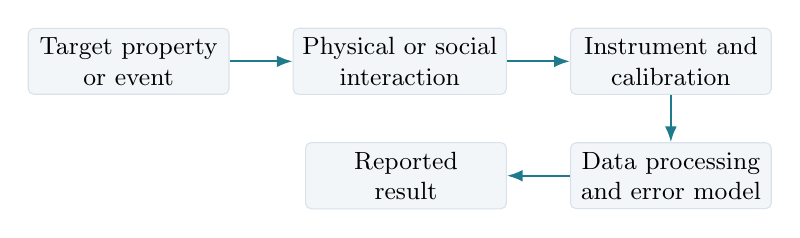
\begin{tikzpicture}[
  node distance=6mm and 8mm,
  box/.style={draw=linegray,rounded corners=2pt,fill=pale,align=center,minimum width=2.55cm,minimum height=0.72cm,font=\small},
  arrow/.style={-{Latex[length=2mm]},draw=teal,thick}
]
\node[box] (target) {Target property\\or event};
\node[box,right=of target] (interaction) {Physical or social\\interaction};
\node[box,right=of interaction] (instrument) {Instrument and\\calibration};
\node[box,below=of instrument] (transform) {Data processing\\and error model};
\node[box,left=of transform] (result) {Reported\\result};
\draw[arrow] (target) -- (interaction);
\draw[arrow] (interaction) -- (instrument);
\draw[arrow] (instrument) -- (transform);
\draw[arrow] (transform) -- (result);
\end{tikzpicture}
\caption{A measurement path. Every arrow is a potential site of error and
also a site where independent validation can be added.}
\label{fig:measurement-path}
\end{figure}

\section{Operationalism and construct validity}

Operationalism insists that a concept should be defined by an operation. The
view has a useful corrective: a definition that cannot guide any procedure is
not yet an empirical concept. But one concept may have several legitimate
operations. Temperature can be measured through expansion, resistance,
radiation, or thermodynamic relations. Intelligence, poverty, and social trust
also admit multiple operationalizations.

An operation is therefore not identical to a definition. It is an instrument
for producing evidence about a construct under conditions. Convergent
measurement asks whether different operations agree when they should.
Discriminant measurement asks whether they remain distinct from neighboring
constructs. Known-group tests ask whether a measure behaves differently in
groups that the theory says should differ. These tests do not eliminate
interpretation, but they distribute it across independent routes.

\section{From data to phenomena}

James Bogen and James Woodward distinguished data from phenomena
\citep{bogenwoodward1988}. Data are local, often noisy records: a set of
instrument readings, images, or observations. Phenomena are stable patterns
that data reveal through analysis, replication, and background knowledge. The
distinction explains why a single observation can be weak evidence while a
robust phenomenon can support a theory.

For example, a particular climate station reading may be affected by
instrument placement, urbanization, or missing values. A long-run warming
pattern is not simply one more reading; it is a phenomenon supported by many
records, corrections, physical mechanisms, and independent indicators. A
single detector event may be ambiguous, while a distribution of events with a
predicted energy relation is a phenomenon.

The distinction also protects against two errors. Data are not automatically
theory-free facts, but phenomena are not inventions of a theory. A phenomenon
is a stabilized pattern that remains identifiable when the routes to it are
varied and criticism is allowed to operate.

\section{Error, uncertainty, and precision}

Precision concerns the spread of repeated measurements. Accuracy concerns
closeness to the target value. A measurement can be precise but systematically
wrong. A model can estimate a tiny standard error because it ignores a major
source of uncertainty. A survey can report many decimal places while its
conceptual validity is poor.

\RCR\ distinguishes three forms of uncertainty.

\begin{itemize}
\item \textbf{Aleatory uncertainty} concerns variation in a process or outcome
that is treated as stochastic for the purpose of analysis.
\item \textbf{Epistemic uncertainty} concerns limited knowledge of parameters,
models, initial conditions, or measurement error.
\item \textbf{Scope uncertainty} concerns whether a result transfers to a
different population, scale, time, or institutional setting.
\end{itemize}

The distinction is not merely terminological. More observations may reduce
sampling uncertainty but do little to correct a biased measurement. A larger
sample may make a misleading operational definition more precise. A model
ensemble may explore parameter uncertainty while leaving structural uncertainty
untouched.

\section{Instrumental realism}

Ian Hacking's emphasis on experimentation suggests a useful form of realism:
instruments can create a stable relation between a target and an effect. But
instrumental success must be unpacked. A detector's output can be used to
control a beam, diagnose a condition, or produce a new phenomenon. The stronger
the independence between the instrument's construction and the claim being
tested, the stronger the resulting support.

One should ask:

\begin{enumerate}
\item Can the result be reproduced with a different instrument principle?
\item Can the calibration be checked against an independent standard?
\item Does the target support interventions that were not used to define it?
\item Do failed attempts reveal a boundary rather than disappear through
post hoc interpretation?
\end{enumerate}

This standard is demanding but not impossible. It is common in metrology,
particle physics, medicine, and engineering. In social research, the analogous
tests may involve alternative measures, preregistered coding, blinded
assessment, administrative records, or natural experiments.

\section{Observation in the social sciences}

Social categories present a special issue because measurement can change the
thing measured. A census category can become an administrative identity. A
test score can alter self-perception. A policy indicator can become a target
that organizations optimize. This does not make the category unreal, but it
means that the measurement relation is reflexive.

\begin{principlebox}
\textbf{Reflexive measurement principle.} When the act of classification can
change behaviour, the measurement path must include feedback from the
classification to the target. Objectivity requires reporting that feedback,
not pretending that the target is static.
\end{principlebox}

Reflexive measurement is one reason why social science needs both causal
models and institutional analysis. A variable can be a real social fact
because people and organizations act on it, while its meaning and effects
depend on rules that can change.

\section*{Chapter summary}

Observation is conceptually mediated but not arbitrary. A measurement becomes
objective to the extent that its path from target to reported result is
traceable, calibrated, error-aware, and open to independent checks. Data are
local records; phenomena are stabilized patterns that survive analysis and
replication. Precision does not guarantee validity, and social measurements
require attention to feedback. Theory and evidence constrain one another
through carefully designed measurement paths.

\begin{discussion}
\begin{enumerate}
\item Which is more dangerous in a measurement: random noise, systematic bias,
or a construct that is poorly defined?
\item Can two measurements of the same construct legitimately disagree?
\item How should a researcher report a result when the target changes in
response to being measured?
\end{enumerate}
\end{discussion}

\begin{furtherreading}
See Hacking (1983) on experiment and intervention, Bogen and Woodward (1988)
on data and phenomena, Sellars (1963) on the critique of the given, and
Frigg and Hartmann (2006) for models and measurement in scientific practice.
\end{furtherreading}


\chapter{Models, Explanation, Prediction, and Laws}
\label{ch:models}

\begin{chapterguide}
Models are treated as selective mediators between theory and world. The
chapter explains how idealized or literally false models can be scientifically
useful, compares major accounts of explanation, and asks what laws of nature
are doing in actual scientific practice. It then connects reduction and
emergence to the idea of scale-specific constraints.
\end{chapterguide}

Scientific theories are rarely used as complete descriptions. Scientists build
models: simplified systems, equations, diagrams, simulations, analogies,
mechanistic sketches, statistical representations, and idealized populations.
A model may contain frictionless planes, perfectly rational agents, isolated
genes, representative households, point particles, or infinite populations.
None of these may exist exactly. Yet the models can reveal dependencies,
generate predictions, and guide interventions.

The philosophical mistake is to treat usefulness and literal truth as
competitors. The right question is what a model represents, under which
transformations, and for which purpose.

\section{Models as mediators}

Mary Morgan and Margaret Morrison describe models as mediators that are
neither simply derived from theory nor copied from the world
\citep{morganmorrison1999}. A model can borrow resources from several
theories, data sources, and experimental practices. It provides a manipulable
object for reasoning.

Ronald Giere's account is similarly selective. A model represents a real system
to a degree and for a purpose when the relevant similarities are identified
\citep{giere1988,giere2004}. A model of a population may represent its age
distribution but not its cultural history. A model of a pendulum may represent
period under small-angle conditions while ignoring air resistance. The model's
success is conditional on what is preserved.

A representation relation is therefore not binary. We can write informally:
\[
  M \xrightarrow[\text{purpose, scale, conditions}]{\text{represents}}
  T,
\]
where \(M\) is a model and \(T\) is a target system. The arrow is labelled
because the same model can represent different features of a target under
different purposes. The representation is strong when relevant relations are
preserved and weak when the model changes the target's behaviour in the
dimension that matters.

\section{Idealization and abstraction}

An idealization deliberately removes factors. Abstraction selects a feature
while leaving other features unspecified. These are not the same. A
frictionless plane removes friction by setting a parameter to zero. A map
abstracts from buildings when it preserves roads and elevation. An agent-based
model may abstract from individual biographies while idealizing agents as
following a simple rule.

A useful idealization should satisfy three conditions.

\begin{enumerate}
\item \textbf{Relevance:} the removed feature should not be central to the
question under investigation.
\item \textbf{Stability:} the result should remain approximately valid when the
removed feature is reintroduced within the intended range.
\item \textbf{Boundary:} the model should state where the idealization breaks
down.
\end{enumerate}

A model can be literally false and structurally accurate. For a simple example,
consider a population model with exponential growth:
\[
  N(t) = N_0 e^{rt}.
\]
Here \(N(t)\) is the population at time \(t\), \(N_0\) is the initial
population, and \(r\) is a constant net growth rate. No real population grows
with an exactly constant \(r\) forever. The model can still represent a local
growth regime, estimate a rate, or provide a baseline against which more
complex models are compared.

The danger is not idealization itself. The danger is forgetting that a result
about the model is being treated as a result about the target without a
transport argument.

\section{Prediction and explanation}

Prediction and explanation overlap but are not identical. A model can predict
an outcome using a reliable correlation without revealing why the outcome
occurs. A mechanism can explain a process without providing a precise long-run
forecast when initial conditions are unknown or the system is chaotic.

The deductive-nomological model associated with Hempel and Oppenheim treats an
explanation as a deduction of the explanandum from laws and initial conditions
\citep{hempeloppenheim1948,hempel1965}. Its great virtue is clarity: it asks
which premises entail the result. Its limitation is that logical derivation
alone does not guarantee explanatory relevance. An irrelevant law can be
included in a valid deduction, and probabilistic explanations do not entail
their outcomes.

Unificationist approaches evaluate explanations by how many phenomena they
derive from a small set of argument patterns. This captures a real value:
compressing unrelated facts into one framework can reveal a shared structure.
But simplicity can mislead when the world is heterogeneous.

Causal and mechanistic approaches focus on how a phenomenon is produced.
Salmon emphasized causal structure and statistical relevance
\citep{salmon1984}. Mechanistic philosophers analyze organized parts and
activities whose interaction produces a behavior
\citep{bechtel2005,craver2007}. These accounts explain why an intervention or
process makes a difference, not only why an equation fits.

\begin{principlebox}
\textbf{Explanatory adequacy principle.} A scientific explanation is adequate
only relative to a question. For a how-question, a mechanism may be required.
For a prediction question, a calibrated statistical model may be enough. For a
why-question about a general pattern, unification or a law-like relation may
matter. No single form of explanation is the universal measure of science.
\end{principlebox}

\section{Laws of nature and local regularities}

A law is often imagined as a universal sentence that describes what nature does
in every circumstance. Actual science is more complicated. Laws may be exact
ideal relations, approximate regularities, symmetry principles, constraints on
possibilities, or statements that hold only under a ceteris paribus clause.

Nancy Cartwright argues that fundamental laws can be highly idealized and that
scientific explanation often proceeds through models that construct a
\enquote{simulacrum} of a phenomenon rather than by direct deduction from
universal laws \citep{cartwright1983,cartwright1999}. This is not a denial of
reality. It is a warning that a law's role in a model may differ from a law's
metaphysical status.

D. M. Armstrong's account treats laws as relations among universals
\citep{armstrong1983}. Other accounts treat them as regularities, dispositions,
or modal constraints. \RCR\ does not settle the ultimate metaphysics by
definition. It says that a law-like claim earns scientific authority when it
captures a stable constraint across a specified range of interventions and
conditions, and when deviations can be explained by additional factors rather
than ignored.

\section{Reduction and emergence}

Reduction has at least three meanings:

\begin{enumerate}
\item \textbf{Ontological reduction:} higher-level entities are nothing over
and above lower-level entities.
\item \textbf{Explanatory reduction:} higher-level laws or explanations can be
derived from lower-level laws.
\item \textbf{Methodological reduction:} a problem is best investigated by
isolating lower-level components.
\end{enumerate}

These meanings can come apart. A social institution may be constituted by
people and rules while still requiring concepts that are not useful in particle
physics. A biological pathway may be physically realized while explanations at
the molecular, cellular, and organismic levels remain distinct. Nagel's
classical model of reduction emphasizes derivation and bridge principles
\citep{nagel1961}; later work has shown that reduction in practice can be
local, approximate, and model-dependent.

Emergence is not a magic word for ignorance. A property is emergent in a
scientifically meaningful sense when it depends on lower-level organization but
has stable patterns, explanatory roles, or causal powers at a higher level.
Phase transitions provide cases where limiting behavior and scale can make
higher-level regularities more informative than a microscopic description
alone \citep{batterman2002}.

\RCR\ treats levels as nested constraint regimes. A higher-level model is not
automatically anti-realist because it cannot be replaced by a lower-level
description in practice. Nor is every higher-level regularity fundamental.
The question is whether the higher-level constraint is stable, manipulable,
and explanatory within its domain.

\section{Simulation and computational models}

Computer simulations are models executed as algorithms. They can explore
systems for which analytic solutions are unavailable, but their results are
not automatically empirical evidence. A simulation inherits assumptions from
its equations, discretization, parameter values, boundary conditions, and
code. It gains epistemic strength when these components are validated against
analytical results, historical data, experiments, or independent simulations.

A simulation can also discover emergent behavior. The discovery is not that
the code produced a surprise in a metaphysical vacuum. It is that a specified
set of rules generates a pattern that was not obvious from inspection and that
can be compared with a target system. The comparison requires a bridge between
the computational state and the phenomenon.

\section{The model's honesty condition}

Every scientific model should make four things visible:

\begin{enumerate}
\item what it treats as the target;
\item what it idealizes or leaves out;
\item which output is a prediction, explanation, or exploratory possibility;
\item how the output was validated and where it should not be transported.
\end{enumerate}

This is the \emph{model's honesty condition}. A model need not contain every
detail to be honest. It needs to distinguish internal consequences from
claims about the world.

\section*{Chapter summary}

Models mediate between theory and world. They are selective, purpose-relative,
and often idealized, but that does not make them arbitrary. A model is
scientifically valuable when it preserves relevant structure, remains stable
under appropriate changes, and states its boundary conditions. Prediction,
explanation, and intervention can come apart. Laws operate through idealized
models and local regimes. Reduction and emergence are best treated as
relations among levels of constraint rather than as all-or-nothing doctrines.

\begin{discussion}
\begin{enumerate}
\item When does an idealization become a distortion rather than a useful
abstraction?
\item Can a model explain a phenomenon if it cannot predict it?
\item Does a higher-level explanation remain objective when a lower-level
description is physically complete?
\end{enumerate}
\end{discussion}

\begin{furtherreading}
See Morgan and Morrison (1999), Giere (1988, 2004), Cartwright (1983, 1999),
Frigg and Hartmann (2006), Salmon (1984), and Craver (2007).
\end{furtherreading}


\chapter{Causality, Mechanisms, and Complexity}
\label{ch:causality}

\begin{chapterguide}
This chapter distinguishes association, intervention, and explanation. It
introduces potential outcomes, directed acyclic graphs, structural causal
models, interventionist explanation, mechanisms, and transportability. The
central claim is that causal knowledge is possible when the inquiry creates or
locates stable constraints on change, not merely patterns of co-occurrence.
\end{chapterguide}

Causal claims answer a practical question: what would happen if something were
changed? A correlation describes how variables vary together. A causal claim
says that a difference in one variable would produce a difference in another
under specified conditions. The distinction is not metaphysical decoration.
Medical treatment, economic policy, education, and climate intervention all
depend on it.

Causality is difficult because the same association can arise from direct
causation, common causes, selection, measurement error, feedback, or chance.
No statistical method can identify a causal interpretation without assumptions
about design, time, variables, and the process generating the data. But the
presence of assumptions does not make causal knowledge impossible. It means
that causal claims should expose the assumptions that make them testable.

\section{Potential outcomes and the missing counterfactual}

The potential-outcomes framework imagines that each unit has an outcome under
each possible treatment. Let \(Y_i(1)\) be the outcome for unit \(i\) if it
receives treatment and \(Y_i(0)\) the outcome if it does not. The individual
causal effect is

\[
  \tau_i = Y_i(1)-Y_i(0).
\]

For a given unit, we observe only one of these two potential outcomes. This is
the fundamental problem of causal inference \citep{rubin1974,holland1986}. A
randomized experiment solves part of the problem by making treatment assignment
independent of potential outcomes in expectation. The average difference
between treatment and control groups can then estimate an average causal
effect, provided the treatment and outcome are defined and measured properly.

Randomization is not a universal substitute for thought. It may have limited
external validity, noncompliance, attrition, spillovers, or ethical
constraints. A trial can estimate what happened under its treatment protocol
without establishing what would happen under a different dose, population, or
institution.

\section{Graphs and confounding}

A directed acyclic graph (DAG) represents assumed causal direction. In a
simple confounding structure, \(C\) affects both treatment \(T\) and outcome
\(Y\):

\begin{figure}[ht]
\centering
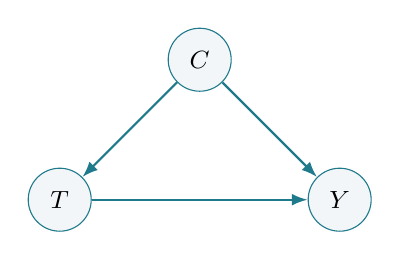
\begin{tikzpicture}[
  node distance=17mm,
  v/.style={draw=teal,fill=pale,circle,minimum size=8mm,font=\small},
  ar/.style={-{Latex[length=2mm]},thick,draw=teal}
]
\node[v] (c) {\(C\)};
\node[v,below left=of c] (t) {\(T\)};
\node[v,below right=of c] (y) {\(Y\)};
\draw[ar] (c) -- (t);
\draw[ar] (c) -- (y);
\draw[ar] (t) -- (y);
\end{tikzpicture}
\caption{A confounding graph: \(C\) is a common cause of treatment \(T\) and
outcome \(Y\). The association between \(T\) and \(Y\) can mix the treatment
effect with the path through \(C\).}
\label{fig:confounding}
\end{figure}

If \(C\) is measured and the graph is credible, conditioning on \(C\) may
block the back-door path from \(T\) to \(Y\). If \(C\) is unmeasured, researchers
may need randomization, an instrumental variable, a natural experiment,
negative controls, sensitivity analysis, or a different design. The graph
does not prove the causal story. It makes the story visible enough to argue
about.

Judea Pearl's structural causal models distinguish observation from
intervention. Informally, \(\Prob(Y\mid T=t)\) describes the outcome among
cases observed with \(T=t\), whereas \(\Prob(Y\mid \doop(T=t))\) describes what
would happen if \(T\) were set to \(t\) by an intervention that removes the
usual causes of treatment \citep{pearl2009}. The distinction explains why an
association can fail to answer a policy question.

\section{Bayesian reasoning about causal claims}

Bayesian reasoning can represent uncertainty about causal hypotheses. Suppose
\(H_1\) says a treatment has a positive effect and \(H_0\) says it has no effect.
The evidence \(E\) changes their odds according to

\[
  \frac{\Prob(H_1\mid E)}{\Prob(H_0\mid E)}
  =
  \frac{\Prob(E\mid H_1)}{\Prob(E\mid H_0)}
  \times
  \frac{\Prob(H_1)}{\Prob(H_0)}.
\]

The first ratio is the likelihood ratio: how much more expected the evidence
is under \(H_1\) than \(H_0\). The second ratio expresses prior odds. A strong
randomized design can make the likelihood ratio informative by reducing
confounding. A weak observational design may produce a large apparent effect
while leaving several causal models compatible with the data.

The equation does not remove causal assumptions. It shows where they enter. A
prior may encode background knowledge about mechanisms. The likelihood depends
on the measurement model, treatment assignment, missingness, and outcome
definition. Good causal inference therefore combines probability with design
and mechanism.

\section{Interventionist explanation}

James Woodward treats causal explanation in terms of stable relations under
interventions \citep{woodward2003}. A variable \(X\) explains a change in \(Y\)
when manipulating \(X\), while holding relevant background conditions fixed,
changes \(Y\) according to a relationship that is stable enough to support
counterfactual reasoning.

This account improves on correlation, but the phrase \enquote{holding fixed}
hides complexity. In a biological system, manipulating one gene may alter many
pathways. In an economy, changing interest rates can trigger expectations and
institutional responses. In a social setting, an intervention can change the
meaning of the variable itself.

\RCR\ therefore adds an \emph{intervention boundary}: a causal claim must state
which variables are changed, which processes are allowed to respond, and which
background conditions are treated as fixed. A causal law is not a universal
promise that every intervention works identically. It is a scope-bound
constraint on a family of interventions.

\section{Mechanisms and causal structure}

Mechanistic explanations describe parts, activities, organization, and the
way their interactions produce a phenomenon. A mechanism is not merely a list
of correlations. It explains how a change propagates through a system.

Mechanistic evidence is especially valuable when it connects different scales.
A drug may bind to a receptor, alter a signaling pathway, change cell behavior,
and improve a clinical outcome. Each link can fail independently. The
mechanistic story is stronger when it is supported by intervention and
measurement at several links rather than inferred from the final outcome alone.

Mechanisms are not always microscopic. A market institution, a school
organization, or a legal procedure can be a mechanism when its parts and rules
produce a stable social outcome. The relevant parts may be persons, norms,
resources, and sanctions rather than molecules.

\section{Complexity, feedback, and nonlinearity}

Complex systems create three challenges for causal inference.

First, effects can be nonlinear. A small change may have little effect below a
threshold and a large effect above it. A linear average can conceal this
structure.

Second, systems can contain feedback. Treatment changes behaviour; behaviour
changes treatment exposure; the outcome changes future measurement. A static
DAG may need to be expanded into a time-indexed graph.

Third, many causes can interact. The effect of an intervention may depend on
context, history, and network position. The average treatment effect can be
scientifically useful while failing to describe any particular subgroup.

These challenges do not defeat objectivity. They make \emph{transportability}
and \emph{heterogeneity} central. A result should be carried to a new setting
only after checking which mechanisms, distributions, and institutional
conditions are shared.

\begin{principlebox}
\textbf{Causal constraint principle.} A causal claim is objective to the degree
that it identifies a stable change-relation supported by design, measurement,
mechanism, or convergent intervention. The claim must state its intervention
boundary and the conditions under which the relation is expected to travel.
\end{principlebox}

\section{What causal knowledge does not require}

Causal knowledge does not require deterministic laws. An intervention can
change a probability distribution without fixing an individual outcome. Nor
does causal knowledge require a single metaphysical definition of cause.
Different sciences may use manipulation, process transmission, counterfactual
dependence, or mechanism construction as complementary modes.

Causal knowledge also does not require the elimination of all uncertainty. It
requires that the uncertainty be attached to a specified causal question. A
claim such as \enquote{this policy works} is too vague. A claim such as \enquote{for
schools with these resources, under this implementation, assignment to this
programme increases average attendance over one year by an estimated range} is
criticizable and therefore epistemically useful.

\section*{Chapter summary}

Correlation records association; causal inference concerns changes under
intervention. Potential outcomes clarify the missing counterfactual, DAGs make
confounding assumptions visible, and structural causal models distinguish
observation from intervention. Mechanisms explain how effects are produced.
Complexity requires attention to nonlinearity, feedback, heterogeneity, and
transportability. \RCR\ treats causal objectivity as the stabilization of
change-relations under explicit intervention boundaries.

\begin{discussion}
\begin{enumerate}
\item Can a randomized trial establish a causal effect if treatment changes
the outcome measure?
\item When is a mechanism more informative than a highly predictive model?
\item How should a causal claim be reported when its average effect hides
opposite effects in subgroups?
\end{enumerate}
\end{discussion}

\begin{furtherreading}
See Rubin (1974), Holland (1986), Pearl (2009), Woodward (2003), Hernan and
Robins (2020), Salmon (1984), and Craver (2007).
\end{furtherreading}


\chapter{Social Epistemology, Standpoints, and Values}
\label{ch:social}

\begin{chapterguide}
This chapter asks whether social location and institutional organization
undermine or improve objectivity. It treats science as a collective achievement,
examines feminist standpoint theory and situated knowledge, and distinguishes
values that select questions from values that distort evidence. The proposed
ideal is public, structured criticism rather than a view from nowhere.
\end{chapterguide}

No individual scientist can reproduce all the measurements, derivations,
computer codes, field observations, and historical records on which a mature
science depends. Scientific knowledge is therefore social in an unavoidable
sense. The question is whether the social character is a source of objectivity,
a source of bias, or both.

The answer is both. Division of labour allows specialization and independent
checking. It also creates authority gradients and dependencies that can hide
errors. Peer review can expose mistakes. It can also enforce conformity.
Funding can support long-term inquiry. It can also redirect attention toward
profitable or politically convenient questions. Social structure is not an
external background to epistemology. It is part of the machinery by which
evidence is produced and evaluated.

\section{The social organization of knowledge}

Social epistemology studies how people pursue truth with and through others.
Alvin Goldman emphasizes testimony, expertise, and the conditions under which
social processes are reliable \citep{goldman1999}. A person often knows
something because another person measured it, and the trustworthiness of that
testimony depends on competence, incentives, access to criticism, and a record
of past performance.

The division of cognitive labour can improve objectivity in at least four ways:

\begin{enumerate}
\item specialists develop techniques too complex for one investigator;
\item independent groups can detect local mistakes;
\item different backgrounds make different anomalies salient;
\item public records allow later investigators to audit procedures.
\end{enumerate}

But social dependence also creates vulnerabilities. A community can coordinate
around a false assumption. A prestigious laboratory can make contrary evidence
hard to publish. Researchers may replicate a result only when it is fashionable.
A field can measure what is easy rather than what is important.

\RCR\ therefore evaluates institutions by their \emph{correction capacity}:
the ability to expose a claim to competent, motivated, and sufficiently
independent criticism. Consensus is evidence only when the process generating
the consensus has a reasonable relation to truth.

\section{Merton's norms and their limits}

Robert Merton described norms associated with the scientific ethos:
communal sharing of knowledge, universalistic assessment, disinterestedness,
and organized skepticism \citep{merton1942}. The norms are ideals, not
descriptions of every laboratory. They express a valuable thought: scientific
claims should be judged by reasons that are not supposed to depend on the
speaker's identity or patronage.

The norms require supplementation. Universalistic assessment can become blind
to how research questions were selected. Communal sharing can conflict with
privacy or intellectual property. Disinterestedness does not mean that
scientists have no values; it means that personal or institutional interests
should not decide the evidential conclusion. Organized skepticism can be
distributed unevenly, with critics demanding impossible standards from
outsiders and weak standards from insiders.

\section{Longino and transformative criticism}

Helen Longino argues that objectivity is not achieved by eliminating social
values from inquiry. It is strengthened by critical interaction under
appropriate social conditions \citep{longino1990}. The relevant conditions
include recognized venues for criticism, uptake of criticism, public
standards, and a degree of equality in intellectual authority.

This account turns disagreement into an epistemic resource. A criticism is not
valuable merely because it is dissenting. It must identify a reason to doubt,
reveal a hidden assumption, offer an alternative, or show that a result does
not travel. The community must also be able to respond rather than ignore the
criticism.

\begin{principlebox}
\textbf{Critical interaction principle.} A scientific community is more
objective when relevant criticism can be expressed, understood, answered, and
incorporated without the critic having to possess the dominant group's
institutional status.
\end{principlebox}

The principle is compatible with expertise. Equality of intellectual authority
does not mean that every claim has equal evidential weight. It means that
access to criticism should not be determined solely by status, and that
expertise itself should be accountable to public reasons.

\section{Standpoint theory and situated knowledge}

Feminist standpoint theory argues that social positions can shape what is
visible and can sometimes provide epistemic advantages concerning relations of
power. Sandra Harding connects standpoint theory to the idea that inquiry
should begin from lives and activities that dominant institutions have treated
as peripheral \citep{harding1991}. Donna Haraway emphasizes situated
knowledges: every perspective is partial, and objectivity requires recognizing
the location and limits of the knower \citep{haraway1988}.

The strongest version is not that every member of an oppressed group
automatically knows the truth. Social position can generate insight, but it
can also generate partiality, pressure, or exclusion. Epistemic advantage is
an achievement of critical reflection and collective inquiry, not a biological
property.

Standpoint insights matter because a theory can fit the experience of a
dominant group while missing the mechanisms affecting others. Research on
workplace safety, medical treatment, domestic labour, disability, and
discrimination can improve when people who bear the consequences participate in
question formation and interpretation. This is not a concession that evidence
is subjective. It is an argument that the range of relevant evidence is
socially organized.

\section{Values in science}

The value-free ideal is ambiguous. There is a legitimate distinction between
values that determine what a result is and values that guide which questions
are worth asking. Scientific work requires choices about significance,
acceptable risk, measurement cost, privacy, classification, and the balance
between false positives and false negatives.

Heather Douglas argues that values can have a legitimate role in decisions
about acceptable error, especially where evidence informs policy
\citep{douglas2009}. Elizabeth Anderson shows how value judgments can guide
concept formation and interpretation without making the evidence itself a
matter of preference \citep{anderson2004}. Max Weber distinguished empirical
analysis from value relevance: values can select a problem without deciding
the factual answer \citep{weber1949}.

\begin{table}[ht]
\centering
\smalltable
\begin{tabularx}{\textwidth}{p{0.28\textwidth}YY}
\toprule
Role of value & Legitimate function & Epistemic risk\\
\midrule
Question selection & Decide what matters to investigate & Neglect of less visible populations\\
Concept formation & Choose distinctions relevant to a problem & Smuggling a conclusion into a definition\\
Loss function & Weigh false positives and false negatives & Treating a policy preference as a fact\\
Evidence interpretation & Decide when uncertainty warrants action & Confirmation bias and motivated reasoning\\
Institutional design & Set rules for access and correction & Exclusion, capture, and authority abuse\\
\bottomrule
\end{tabularx}
\caption{Values can enter different stages of inquiry. Their presence does not
make all stages subjective, but it makes transparency necessary.}
\label{tab:values}
\end{table}

The key distinction is between \emph{constitutive} and \emph{evidential}
values. Constitutive values help determine what to study, how to measure it,
and what risks to accept. Evidential values would make a claim count as true
because it serves an interest, regardless of the evidence. The first are
unavoidable and can be legitimate. The second corrupt objectivity.

\section{When institutions corrupt inquiry}

A research system becomes less objective when it systematically weakens the
routes by which errors can be found. Warning signs include:

\begin{itemize}
\item selective publication and undisclosed outcome switching;
\item opaque data processing and unavailable code;
\item conflicts of interest that affect design or interpretation;
\item exclusion of relevant populations from research;
\item status-based dismissal of criticism;
\item incentives that reward novelty while penalizing correction.
\end{itemize}

These are not merely ethical defects. They are epistemic defects because they
alter what evidence becomes visible and how it is weighted. A conflict of
interest does not prove a conclusion false, but it changes the expected
reliability of the process and should trigger stronger independent checks.

\section{Objectivity as social self-correction}

The view from nowhere is impossible. A more realistic ideal is a community that
can locate its own partiality. \RCR\ calls this \emph{reflexive objectivity}.
It has four components:

\begin{enumerate}
\item the perspective and values of inquiry are stated;
\item affected and relevantly situated people can challenge the framing;
\item independent criticism can inspect the evidence and analysis;
\item revisions are judged by their improved contact with the target, not only
by their political convenience.
\end{enumerate}

Reflexive objectivity is not guaranteed by diversity alone. A diverse group can
share the same measurement error. Nor is objectivity guaranteed by
disinterestedness alone. A narrow research agenda can be very carefully
pursued. The point is to connect social inclusion with world-directed tests.

\section*{Chapter summary}

Scientific knowledge is socially produced, and social organization can improve
or corrupt objectivity. Division of labour, expertise, criticism, and public
records create correction capacity. Merton's norms are valuable ideals but
require attention to power and question selection. Longino, Harding, and
Haraway show why critical pluralism and situated perspectives can reveal
ignored phenomena. Values legitimately shape questions, concepts, risk
thresholds, and institutions; they should not decide evidential conclusions by
fiat. Objectivity is therefore reflexive: it includes the ability of inquiry to
expose its own partiality.

\begin{discussion}
\begin{enumerate}
\item Is a scientific community objective if it is highly diverse but has no
effective correction mechanisms?
\item Which values should be public in a medical or policy study?
\item How can standpoint insights be tested without reducing them to identity
claims?
\end{enumerate}
\end{discussion}

\begin{furtherreading}
Read Longino (1990), Harding (1991), Haraway (1988), Anderson (2004),
Douglas (2009), Goldman (1999), and the literature on social dimensions of
scientific knowledge.
\end{furtherreading}


\chapter{Uncertainty, Replication, and Demarcation}
\label{ch:reliability}

\begin{chapterguide}
This chapter examines how scientific systems learn from error. It compares
Bayesian and error-statistical approaches, explains why replication is more
than repeating a number, and develops a functional account of demarcation.
The goal is not certainty, but reliable correction under uncertainty.
\end{chapterguide}

Fallibility is not a defect that science can eliminate. It is a condition that
science can manage better or worse. A reliable inquiry does not promise that
its claims are never wrong. It makes it possible to discover where they are
wrong, how much depends on them, and what should replace them.

This shift matters because scientific reliability is often discussed as if one
test could settle it. A \(p\)-value, a confidence interval, a Bayesian
posterior, a replication, or an expert consensus can each be informative. None
is self-interpreting. Objectivity lies in the relation among design, error
control, evidence, and revision.

\section{Probability as rational change}

Bayesian epistemology gives a precise rule for coherent belief revision. For
hypothesis \(H\) and evidence \(E\),

\[
  \Prob(H\mid E)
  =
  \frac{\Prob(E\mid H)\Prob(H)}{\Prob(E)}.
\]

The rule has two virtues. It forces the investigator to compare a hypothesis
with alternatives, and it distinguishes evidence from belief. The likelihood
\(\Prob(E\mid H)\) is not the same as the posterior probability
\(\Prob(H\mid E)\). A surprising result can be strong evidence for \(H\) over
\(H_0\) even when \(H\) remains improbable in an absolute sense.

The rule has limits. Priors can encode relevant background knowledge, but they
can also encode unjustified assumptions. Likelihoods depend on the model of
data collection and analysis. If an investigator tests many hypotheses and
reports only the surprising one, the reported evidence does not have the
likelihood that a preregistered test would have had.

\section{Error-statistical learning}

Deborah Mayo emphasizes learning from error: a result is informative when a
procedure would probably have produced a different result if a relevant error
were present \citep{mayo1996}. This is a frequentist and experimental
complement to Bayesian reasoning. It focuses on how a design probes error
rather than on the subjective degree of belief in a hypothesis.

The two approaches need not be enemies. Bayesian updating answers how beliefs
should change given a specified model. Error-statistical analysis asks whether
the procedure has good capability to detect errors or discrepancies. \RCR\
uses both as diagnostic tools:

\begin{itemize}
\item use likelihoods and priors to compare claims transparently;
\item use error analysis to ask what the design would have detected;
\item report model uncertainty and the possibility that the analysis was
selected after seeing the data.
\end{itemize}

\section{Replication is not a magic word}

A replication repeats a study or result under some relation of similarity.
There are several kinds:

\begin{enumerate}
\item \textbf{Exact replication:} repeats procedures as closely as possible.
\item \textbf{Conceptual replication:} tests the same claim using a different
operationalization or design.
\item \textbf{Robustness test:} changes a condition that should not matter if
the mechanism is stable.
\item \textbf{Extension:} tests whether the claim travels to a new population,
scale, or context.
\end{enumerate}

A failed replication can have several interpretations. The original effect may
be false, the replication may have lower power, the procedures may differ in a
causally relevant way, the effect may be context-sensitive, or the original
estimate may have been inflated by selection. The correct response is not to
declare a field true or false from one replication rate. It is to inspect the
conditions under which the effect appears.

The Open Science Collaboration's 2015 project attempted replications of 100
psychological studies. It reported that replicated effects were, on average,
smaller than original effects and that there was no single standard for
replication success \citep{osc2015}. The study is valuable precisely because
its interpretation requires more than one headline number. It reveals how
publication selection, statistical power, measurement, and context interact.

\section{Uncertainty and the replication ladder}

\RCR\ proposes a replication ladder. A claim receives stronger support as it
survives increasingly independent challenges:

\begin{enumerate}
\item reanalysis of the same data;
\item independent code or analytical pipeline;
\item new data with the original design;
\item different measurement or instrument;
\item different population or setting;
\item intervention on the mechanism;
\item use in a successful new prediction or application.
\end{enumerate}

The ladder is not a demand that every claim reach the final rung. A historical
claim may not permit intervention. A mathematical theorem has a different
structure. A medical treatment may be ethically tested only within a narrow
population. The ladder is a way to specify what kind of support has been
achieved, not a universal ranking of sciences.

\section{The demarcation problem}

The demarcation problem asks how to distinguish science from non-science or
pseudoscience. Popper proposed falsifiability. Lakatos emphasized progressive
problem shifts. Laudan argued that the search for a single demarcation
criterion had failed and that the more useful question is whether claims are
reliable, problem-solving, and evidentially supported \citep{laudan1977,laudan1983}.

A binary boundary is attractive for public decisions, but scientific practices
are too diverse for one property to do all the work. Some mature sciences make
few direct predictions; some non-scientific practices generate testable
predictions. A field can be methodologically serious in one period and
degenerate in another.

\RCR\ replaces a single boundary with a profile of epistemic performance. A
claim or practice is more science-like when it:

\begin{itemize}
\item creates risky contact with a target;
\item records methods, data, and uncertainty;
\item exposes itself to independent criticism;
\item updates or abandons claims when evidence requires it;
\item separates empirical results from value and metaphysical interpretation;
\item supports transportable predictions, interventions, or explanations.
\end{itemize}

This is a functional demarcation criterion. It does not say that science is
whatever produces useful outcomes. It says that the institutional practice
deserves scientific authority to the extent that it maintains correction
capacity under world-sensitive constraints.

\section{Scientism and the misuse of science}

Scientism is not simply confidence in science. It is the unwarranted extension
of scientific authority beyond the question, method, or evidence that supports
it. A physical law does not by itself determine an ethical obligation. A
statistical regularity does not settle a political priority. A model of human
behaviour does not eliminate interpretation, meaning, or agency.

\RCR\ rejects scientism for the same reason it rejects relativism: both
collapse distinctions. Science is authoritative for claims that its methods
can constrain. It is not a universal replacement for history, ethics,
political judgment, or lived interpretation. This limitation protects science
from being asked to prove what its methods cannot address, and protects other
forms of reasoning from being dismissed by an illegitimate appeal to scientific
status.

\section{Reliability as a system property}

A single true claim can emerge from an unreliable process by luck. A single
false claim can emerge from a generally reliable process by chance. The
objectivity of science is therefore not exhausted by the truth value of
individual outputs. It includes the design of a system that tends to correct
errors over time.

A system's reliability depends on:

\begin{enumerate}
\item the quality of its measurements and models;
\item the independence and competence of its critics;
\item the incentives attached to novelty and correction;
\item the visibility of negative results and failed replications;
\item the capacity to revise concepts, not only parameter estimates.
\end{enumerate}

The fifth point is crucial. A field can replicate a measurement reliably while
measuring the wrong construct. Objectivity sometimes requires changing the
question.

\begin{principlebox}
\textbf{Correction principle.} The epistemic standing of a scientific claim
depends not only on present support but on the quality of the process that
could reveal its failure. A claim with moderate evidence and strong correction
capacity can be more trustworthy than a claim with impressive evidence inside
an opaque and uncorrectable system.
\end{principlebox}

\section*{Chapter summary}

Probability formalizes belief revision; error statistics asks what a procedure
could have detected; replication tests stability under controlled variation;
and demarcation is best understood as a profile of correction capacity rather
than one binary test. Scientific authority should be proportional to the
quality of world-sensitive error correction. This supports fallibilism without
relativism and confidence without scientism.

\begin{discussion}
\begin{enumerate}
\item When does a failed replication count against a claim?
\item Is a transparent but imperfect method preferable to a highly accurate
method whose assumptions cannot be inspected?
\item Can a practice be scientific in one domain and non-scientific in another?
\end{enumerate}
\end{discussion}

\begin{furtherreading}
See Mayo (1996), the Open Science Collaboration (2015), Ioannidis (2005),
Laudan (1977, 1983), and Reiss and Sprenger (2014).
\end{furtherreading}


\chapter{The Ontology of Reflexive Constraint Realism}
\label{ch:ontology}

\begin{chapterguide}
This chapter states the ontological side of Reflexive Constraint Realism
(\RCR). It defines reality, entities, processes, structures, laws, levels, and
social facts, then gives the framework's axioms and graded commitment ladder.
The aim is a defensible realism that does not pretend that science supplies a
complete inventory of being.
\end{chapterguide}

\RCR\ begins with a modest but non-negotiable ontological claim: the world does
not depend on human inquiry for its existence. Stars existed before astronomy.
Biological reproduction preceded genetics. People and institutions can affect
one another before social scientists classify them. A mind-independent world is
not necessarily a world described by one final vocabulary. It is a world whose
behaviour can resist, frustrate, and correct our descriptions.

The word \emph{constraint}\index{constraint} is central. A constraint is a
stable restriction on what can happen, or a stable tendency that makes some
changes more likely than others, under specified conditions. A wall constrains
motion. A chemical bond constrains molecular configurations. A legal rule
constrains behaviour through sanctions and expectations. A statistical
relationship can express a constraint when it remains stable under relevant
changes. The concept is broad enough to travel across sciences but precise
enough to require a scope.

\section{Generative reality}

The ontology of \RCR\ is \emph{generative}: reality contains processes that
produce events, not only a collection of regular sequences. A mechanism, field,
institution, or ecological relation matters because it makes a difference to
what can happen. Generativity does not require determinism. A stochastic
process can generate a distribution. A social institution can make behaviour
more likely without forcing each individual action.

The ontology is also \emph{layered}. Physical processes, organisms, persons,
institutions, and ecosystems can be dependent on one another without being
interchangeable descriptions. A higher-level entity is real when it has
stable powers, boundaries, or relations that make a difference to outcomes,
even if it is physically realized by lower-level processes.

Finally, the ontology is \emph{open}. Science may discover new kinds of entity,
and current categories may be replaced. The framework should therefore state
what warrants commitment without claiming to know the final catalogue of
reality.

\section{Eight axioms}

The following axioms are methodological-metaphysical starting points. They are
not self-evident truths from which all science can be deduced. They are
commitments that make the project of objective inquiry intelligible and expose
where it can fail.

\begin{principlebox}
\textbf{Axiom 1: Mind-independent generativity.} There is a reality whose
processes do not depend for their existence on being represented by human
agents. Those processes generate resistances, regularities, possibilities, and
events that inquiry can discover imperfectly.
\end{principlebox}

\begin{principlebox}
\textbf{Axiom 2: Constraint plurality.} The world constrains inquiry through
more than one kind of relation: material interaction, causal production,
mathematical structure, temporal dependence, ecological organization, and
social rule. No single layer is assumed to exhaust all scientifically relevant
being.
\end{principlebox}

\begin{principlebox}
\textbf{Axiom 3: Mediated access.} Scientific access to reality is always
mediated by concepts, instruments, models, language, and institutions. Mediation
does not imply invention; it creates a route through which independent
constraints can act on claims.
\end{principlebox}

\begin{principlebox}
\textbf{Axiom 4: Fallibility.} Every finite scientific claim is revisable.
Confidence can be high without being certain, and ontological commitment can
be strong without being final.
\end{principlebox}

\begin{principlebox}
\textbf{Axiom 5: Invariance matters.} A claim gains epistemic and ontological
support when its relevant consequences remain stable under admissible changes
of observer, instrument, representation, intervention, or context.
\end{principlebox}

\begin{principlebox}
\textbf{Axiom 6: Situated inquiry.} Every inquiry begins from a location in a
social, material, and historical system. The location affects what becomes
visible, but it need not determine what is true.
\end{principlebox}

\begin{principlebox}
\textbf{Axiom 7: Public corrigibility.} Objective inquiry requires practices
through which competent others can inspect, challenge, reproduce, and revise a
claim. Private certainty is not a substitute for public correction.
\end{principlebox}

\begin{principlebox}
\textbf{Axiom 8: Scope-bound truth.} A claim is true only with respect to the
objects, variables, scales, interventions, and background conditions that its
evidence supports. Generality must be earned by transport.
\end{principlebox}

Axioms 1 and 3 must be held together. If one accepts only Axiom 1, one risks
naive realism: the world is real, so observations are treated as transparent.
If one accepts only Axiom 3, one risks constructivist relativism: all access is
mediated, so reality becomes indistinguishable from representation. Axioms 5
through 8 explain how mediation can be disciplined.

\section{What scientific entities are}

An entity is not simply whatever appears as a noun in a theory. \RCR\ uses
three tests.

\begin{enumerate}
\item \textbf{Boundary test:} Can the entity be distinguished from neighbouring
processes by a stable criterion?
\item \textbf{Difference test:} Does changing or removing the entity make a
reliable difference to outcomes?
\item \textbf{Convergence test:} Do independent measurements, models, or
interventions support the entity's role?
\end{enumerate}

An entity can pass these tests without being fundamental. A gene may be a
molecular sequence, a regulatory function, or a population-level unit depending
on the question. A firm is not a biological organism, but it can be a real
social entity if it has legally recognized boundaries, resources, decision
procedures, and causal effects.

\RCR\ therefore distinguishes \emph{realization} from \emph{reduction}. To say
that a higher-level entity is realized by lower-level processes is to say that
the higher-level entity depends on them. To say that it is reducible is to say
that its explanatory and causal role can be replaced without loss. The first
does not entail the second.

\section{Structures and relations}

A structure consists of elements together with relations and transformations.
Scientific theories often support relations more strongly than they support
the intrinsic nature of elements. A model may establish that changes in \(X\)
alter \(Y\) with a certain pattern without determining whether \(X\) is a
fundamental property or a useful aggregate.

The realist commitment to structure must be disciplined by relevance. A
mathematical isomorphism alone does not show that two physical systems share
the same ontology. The relation must survive a mapping between model and
target, and it must matter to prediction, intervention, or explanation.

\section{Laws as modal constraints}

\RCR\ treats laws of nature as candidates for stable modal constraints: they
describe what would happen under a range of admissible changes, not merely what
has happened so far. A law-like claim can be probabilistic, approximate, or
scale-specific. It becomes law-like when its counterfactual and interventional
consequences are stable enough to guide inquiry.

This view avoids the choice between universal regularity and mere description.
A law can be a real feature of a domain without being the only law that exists
or without applying outside the regime in which its variables are well-defined.

\section{The ontology of social facts}

Social facts are not less real because they depend on human activity. Money,
property, citizenship, corporations, and scientific institutions have histories
and rules, but they constrain behaviour and distribute resources. Their
existence is relational and reflexive: they persist because people recognize,
enforce, or enact them, yet once established they are not freely adjustable by
each individual.

The ontology of social science must therefore include at least:

\begin{itemize}
\item material bodies and environments;
\item agents with capacities and interpretations;
\item rules, norms, and institutions;
\item networks of dependence and power;
\item historical trajectories that alter future possibilities.
\end{itemize}

A social explanation should not collapse a norm into a molecule, but neither
should it detach the norm from the people, artifacts, and sanctions that
realize it.

\section{Graded ontological commitment}

\RCR\ recommends a commitment ladder. The ladder is not a probability scale.
It records what sort of support has been earned.

\begin{table}[ht]
\centering
\smalltable
\begin{tabularx}{\textwidth}{p{0.25\textwidth}Y Y}
\toprule
Level & Commitment & Typical warrant\\
\midrule
L0: useful posit & Use the term without belief in its independent reality & Predictive or computational utility\\
L1: empirical pattern & Believe that a stable phenomenon occurs & Convergent measurement and replication\\
L2: structural commitment & Believe that a relation or invariance is real in a domain & Cross-model stability and limiting relations\\
L3: causal commitment & Believe that an entity, process, or mechanism makes a difference & Intervention, counterfactual robustness, mechanism\\
L4: domain ontology & Treat a family of entities and relations as real in a mature domain & Long-run convergence, transport, integration, and correction\\
\bottomrule
\end{tabularx}
\caption{The \RCR\ commitment ladder. Movement upward requires stronger and
more independent constraints; movement downward remains possible after
counterevidence.}
\label{tab:commitment-ladder}
\end{table}

The ladder protects against two errors. It prevents a useful model from being
treated as a literal inventory. It also prevents anti-realism from ignoring
the epistemic significance of interventions that could not succeed if the
relevant entity or structure were absent.

\section{A layered map of reality}

\begin{figure}[ht]
\centering
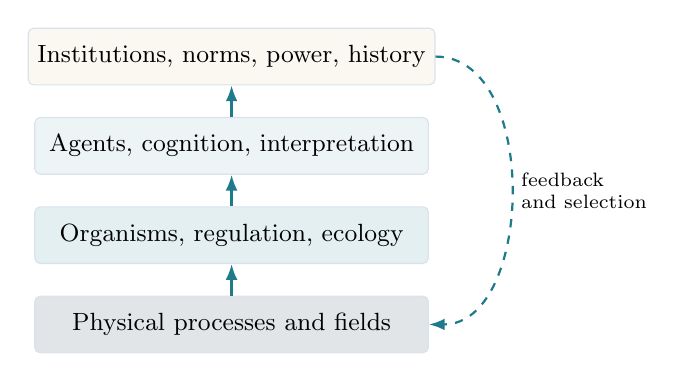
\begin{tikzpicture}[
  layer/.style={draw=linegray,rounded corners=2pt,align=center,minimum width=5.0cm,minimum height=0.72cm,font=\small},
  ar/.style={-{Latex[length=2mm]},draw=teal,thick}
]
\node[layer,fill=covernavy!12] (phys) {Physical processes and fields};
\node[layer,fill=teal!12,above=4mm of phys] (bio) {Organisms, regulation, ecology};
\node[layer,fill=teal!8,above=4mm of bio] (agent) {Agents, cognition, interpretation};
\node[layer,fill=warm,above=4mm of agent] (soc) {Institutions, norms, power, history};
\draw[ar] (phys) -- (bio);
\draw[ar] (bio) -- (agent);
\draw[ar] (agent) -- (soc);
\draw[ar,dashed] (soc.east) to[out=0,in=0] node[right,font=\scriptsize,align=left]{feedback\\and selection} (phys.east);
\end{tikzpicture}
\caption{A non-reductive layered ontology. Higher layers are realized by lower
processes while feeding back through organization, action, and selection.}
\label{fig:ontology-layers}
\end{figure}

The diagram is not a ladder of value or a claim that reality has exactly four
levels. It is a reminder that scientific explanations can move across levels.
A social institution is materially realized, psychologically interpreted, and
historically reproduced. A disease is biological, embodied, measured, and
institutionally classified. Objectivity depends on preserving the causal links
between levels rather than pretending that one level can answer every question.

\section*{Chapter summary}

\RCR\ posits a mind-independent, generative, layered, and open reality. Its
basic unit is the constraint: a stable restriction or tendency that survives
specified changes. Entities earn commitment through boundary, difference, and
convergence tests. Structures are real when relevant relations remain stable
across representations and interventions. Laws are modal, scope-bound
constraints. Social facts are real relational entities. The eight axioms and
the commitment ladder make realism graded, fallible, and accountable.

\begin{discussion}
\begin{enumerate}
\item Can an entity be real without being fundamental?
\item What would count as evidence that a higher-level social mechanism has
causal powers?
\item Does the commitment ladder describe degrees of belief, degrees of truth,
or degrees of warrant?
\end{enumerate}
\end{discussion}

\begin{furtherreading}
Compare the layered approach here with Chakravartty (2007), Cartwright (1999),
Craver (2007), Batterman (2002), Oppenheim and Putnam (1958), and the
literature on reduction and emergence.
\end{furtherreading}


\chapter{The Epistemology of Reflexive Constraint Realism}
\label{ch:epistemology}

\begin{chapterguide}
This chapter gives \RCR\ an epistemology. It defines evidence, states
inferential rules, explains how belief should change, and proposes criteria for
comparing theories. The framework does not replace Bayesian, causal,
experimental, or interpretive methods; it specifies how their results can be
assembled into an objective but fallible claim.
\end{chapterguide}

The ontological claim that reality constrains inquiry is not enough. A world can
be real while our beliefs about it are systematically wrong. \RCR's
epistemology therefore asks how constraints become reasons. A reason is not
simply an event that occurs before belief. It is evidence when the event
discriminates among claims under a defensible measurement and inferential
model.

\section{Claims, targets, and alternatives}

Every scientific claim should be represented with five fields:

\begin{enumerate}
\item \textbf{Target:} the entity, process, relation, or population at issue;
\item \textbf{content:} what is being asserted about the target;
\item \textbf{scope:} the time, place, scale, population, and intervention
conditions;
\item \textbf{alternatives:} rival explanations or models;
\item \textbf{warrant:} the evidence and reasoning supporting the claim.
\end{enumerate}

A sentence such as \enquote{\(X\) causes \(Y\)} is incomplete. It does not say
which \(X\), which \(Y\), in what population, by what intervention, or against
which confounders. A scoped claim can be tested. A vague claim can survive by
changing its meaning.

\section{Evidence as constraint}

Evidence \(E\) supports a claim \(H\) when \(E\) is more expected under \(H\)
than under relevant alternatives, or when \(E\) forces a revision of those
alternatives. The Bayesian expression is the likelihood ratio:

\[
  \operatorname{LR}(E;H_1,H_0)
  =
  \frac{\Prob(E\mid H_1)}{\Prob(E\mid H_0)}.
\]

A likelihood ratio greater than one favours \(H_1\) over \(H_0\); a ratio less
than one favours \(H_0\). The ratio does not establish either hypothesis as
true. It measures the evidential direction and strength relative to a model.

In practice, \(\Prob(E\mid H)\) includes assumptions about sampling,
measurement, missingness, and analysis. \RCR\ therefore requires that the
evidence statement carry its measurement path and scope conditions with it.

\begin{principlebox}
\textbf{Evidence rule.} Do not ask whether a result is evidence in isolation.
Ask: evidence for which claim, against which alternative, under which
measurement path, and with what expected error if the claim were false?
\end{principlebox}

\section{The inferential rules}

The following rules are the operational core of \RCR. They are norms for
reasoning, not algorithms that mechanically settle every case.

\begin{enumerate}[label=\textbf{R\arabic*.}]
\item \textbf{Scope before strength.} State the claim's target and scope before
assigning confidence. A highly precise claim with an undefined target has
little epistemic content.
\item \textbf{Path traceability.} Trace the path from target to datum to
conclusion. Separate observation, transformation, model assumption, and
interpretation.
\item \textbf{Alternative exposure.} Compare a claim with serious alternatives.
A result that fits \(H\) but also fits many rivals has limited discriminating
force.
\item \textbf{Risk preference.} Prefer tests that create outcomes likely to
differ across hypotheses. Confirmation is stronger when the test was not
designed to guarantee success.
\item \textbf{Invariance search.} Vary observers, instruments, operational
definitions, samples, models, or interventions where the claim says the
result should remain stable.
\item \textbf{Causal separation.} Do not infer causal adequacy from predictive
fit alone. Require design, intervention, mechanism, or a clearly defended
counterfactual model.
\item \textbf{Transport discipline.} Do not move a result to a new setting
without identifying shared mechanisms and checking changed distributions.
\item \textbf{Commitment proportionality.} Match ontological commitment to the
strongest layer of evidence actually established.
\item \textbf{Revision readiness.} State what evidence would lower confidence or
change the model. A claim insulated from revision is not strengthened by
confidence.
\item \textbf{Social accountability.} Treat competent, relevant criticism as a
source of information about hidden assumptions, not merely as a political
obstacle.
\end{enumerate}

The rules can conflict. A high-risk test may be unethical. An exact replication
may be impossible. A new operationalization may alter the target. In such
cases, the conflict should be reported rather than hidden. \RCR\ is a framework
for making trade-offs visible, not a claim that every trade-off has one
correct answer.

\section{Belief revision}

Belief revision should be continuous, comparative, and calibrated. Continuous
does not mean that all beliefs must be represented by exact numbers. It means
that the language of confidence should reflect degrees of support. Comparative
means that confidence in one claim depends on how it performs against
alternatives. Calibrated means that predictions are checked against outcomes.

A useful reporting format separates:

\begin{itemize}
\item prior background assumptions;
\item new evidence;
\item the likelihood or expected error under each alternative;
\item the updated confidence;
\item remaining uncertainty and scope limitations.
\end{itemize}

This format is compatible with Bayesian updating, confidence intervals,
likelihoodist reasoning, error statistics, or qualitative comparative
inference. The common requirement is that the route from evidence to belief be
auditable.

\section{Theory comparison}

Theories should not be ranked by one virtue alone. A simple theory can be too
simple. A detailed theory can overfit. A highly predictive theory can lack a
causal mechanism. A metaphysically rich theory can make no risky difference.

\RCR\ proposes a comparative profile with seven dimensions:

\begin{enumerate}
\item empirical fit to established phenomena;
\item novel or risky success;
\item structural and causal coherence;
\item robustness under independent changes;
\item explanatory reach and integration;
\item simplicity relative to scope and complexity;
\item transparency, corrigibility, and transportability.
\end{enumerate}

For an informal representation, let a theory \(T\) have profile
\[
  \mathbf{V}(T) =
  (F,N,C,R,X,S,O),
\]
where the letters stand for fit, novelty, coherence, robustness, explanatory
reach, simplicity, and objectivity of process. The profile is not a single
score. In some decisions one dimension can dominate: a medical treatment may
require safety even if its explanatory theory is incomplete. In others,
structural coherence or novel prediction may matter more.

A weighted score can be used when a purpose requires one:
\[
  Q(T) = \sum_{j=1}^{7} w_j V_j(T),
  \qquad
  w_j \geq 0,\quad \sum_{j=1}^{7}w_j=1.
\]
Here \(w_j\) are explicit weights chosen for a stated purpose. The equation
does not create objectivity by arithmetic. It prevents hidden trade-offs from
masquerading as neutral judgment.

\begin{table}[ht]
\centering
\smalltable
\begin{tabularx}{\textwidth}{p{0.22\textwidth}Y Y}
\toprule
Dimension & Strong performance & Typical warning sign\\
\midrule
Fit & Accounts for reliable phenomena within error & Selective use of data\\
Novelty & Predicts or reveals outcomes not used to tune the theory & Post hoc accommodation\\
Coherence & Links mechanisms, equations, and concepts without contradiction & Ad hoc patches\\
Robustness & Survives instruments, samples, and model changes & Fragility to one pipeline\\
Reach & Connects domains or scales with clear bridges & Vague unification\\
Simplicity & Achieves scope without needless complexity & Underfitting or oversimplification\\
Process objectivity & Makes criticism and revision possible & Opaque methods or status protection\\
\bottomrule
\end{tabularx}
\caption{A comparative profile for theory choice. No dimension is sufficient on
its own.}
\label{tab:theory-profile}
\end{table}

\section{Explanation and evidence are distinct}

A theory may explain a phenomenon but fit data poorly because the measurements
are noisy. A statistical model may fit and predict accurately without
identifying the mechanism. A mechanism may be true while a quantitative
parameter is wrong. \RCR\ avoids forcing these into one score by reporting
separate warrants.

This distinction is also useful for scientific communication. A paper should
not describe an associational analysis as a causal explanation merely because
the proposed story is plausible. It should not describe a computational
possibility as an empirical prediction until the bridge to the target is
identified. It should not describe a normatively preferred outcome as a
scientific conclusion without separating values from evidence.

\section{Objectivity criteria}

A claim qualifies as objective in the \RCR\ sense when it satisfies the
following criteria to a degree appropriate to its field:

\begin{enumerate}
\item \textbf{World resistance:} the claim confronts effects that investigators
cannot freely choose.
\item \textbf{Cross-perspective convergence:} relevantly different observers or
methods identify the same pattern.
\item \textbf{Measurement accountability:} the path from target to result is
traceable and error-aware.
\item \textbf{Intervention or counterfactual grip:} the claim supports a
well-defined change relation where one is possible.
\item \textbf{Model transparency:} idealizations and bridge assumptions are
stated.
\item \textbf{Critical independence:} competent others can inspect and challenge
the claim.
\item \textbf{Scope honesty:} the claim does not travel further than its
evidence.
\item \textbf{Revision capacity:} the inquiry can detect and incorporate error.
\end{enumerate}

These criteria are not a checklist that produces certainty. They are dimensions
along which a research system can improve. A claim may score strongly on
measurement and weakly on intervention because the target is historical. It may
score strongly on causal grip and weakly on transport because the setting is
unique.

\section{What makes the epistemology reflexive}

Reflexivity means more than adding a disclaimer about bias. It requires
studying how the inquiry's own categories and procedures change the target,
the evidence, or the community. In social science, a classification can
become an incentive. In medicine, a diagnostic label can affect treatment. In
physics, a detector design defines which events are accessible. In all cases,
the inquiry should ask what it has made visible and what it has excluded.

A reflexive epistemology is not self-defeating. The fact that an inquiry has
conditions does not imply that its conclusions are only about those conditions.
It means that a conclusion earns broader authority when it survives changes to
the conditions that are not supposed to matter.

\section*{Chapter summary}

\RCR\ treats evidence as a claim-relative constraint, not as a free-floating
fact. Its ten inferential rules require scope, traceability, alternatives,
risk, invariance, causal separation, transport discipline, proportional
commitment, revision readiness, and social accountability. Theory comparison
uses a profile of fit, novelty, coherence, robustness, reach, simplicity, and
process objectivity. The criteria of objectivity are graded, field-sensitive,
and designed to make error discoverable.

\begin{discussion}
\begin{enumerate}
\item Should a theory with stronger fit but weaker causal explanation be
preferred for prediction?
\item Which of the ten rules is most difficult to satisfy in social science?
\item Can explicit values improve theory comparison rather than bias it?
\end{enumerate}
\end{discussion}

\begin{furtherreading}
Compare the updating logic here with Bayes (1763), Reichenbach (1938), Mayo
(1996), and the causal frameworks of Pearl (2009) and Woodward (2003).
\end{furtherreading}


\chapter{Scientific Progress and Theory Choice}
\label{ch:progress}

\begin{chapterguide}
This chapter asks in what sense science progresses if theories are revised and
models are idealized. It distinguishes accumulation from improvement, considers
underdetermination and unconceived alternatives, and explains how \RCR\ treats
theory change as the enlargement and stabilization of constraint-sensitive
inference.
\end{chapterguide}

If objectivity is fallible, what makes one theory better than another? A later
theory may be less simple, less intuitive, or less familiar. It may reject
entities once considered real. It may also predict more accurately, explain
more phenomena, support new interventions, and clarify its own limitations.
Scientific progress is not the absence of change. It is change that increases
the reliability, range, precision, or depth of inquiry.

\section{Against simple accumulation}

The accumulation picture says that science adds facts to a fixed stock of
knowledge. Kuhn showed why this is inadequate: revolutions change concepts,
problems, and standards \citep{kuhn1962}. But the opposite picture, in which
each theory is a self-contained world, is also inadequate. Later science often
preserves measurements, limiting cases, mathematical relations, instruments,
and practical controls.

\RCR\ identifies five forms of progress:

\begin{enumerate}
\item \textbf{Empirical progress:} more reliable phenomena are established and
fewer important results remain unexplained.
\item \textbf{Predictive progress:} the theory yields new, risky, and calibrated
predictions.
\item \textbf{Causal progress:} the theory identifies more stable mechanisms
and intervention boundaries.
\item \textbf{Representational progress:} models preserve relevant structure
across wider ranges or provide better approximations.
\item \textbf{Reflexive progress:} the inquiry becomes better at identifying
its own errors, assumptions, and social exclusions.
\end{enumerate}

These dimensions can conflict. A more accurate model may be less interpretable.
A broader theory may weaken local fit. A new measure may reveal that an old
effect was an artifact. Progress is therefore multidimensional and must be
reported as a profile.

\section{The problem of underdetermination}

For any finite set of observations, many models may fit. This is
underdetermination. It follows from the fact that data constrain hypotheses
but do not usually select one uniquely. Duhem's holism and Quine's web of
belief make the problem vivid \citep{duhem1906,quine1951}.

The existence of alternatives does not imply that theory choice is arbitrary.
Researchers can generate new constraints by measuring a different variable,
designing a discriminating experiment, comparing interventions, or testing
novel domains. The appropriate response to underdetermination is not to
declare victory for the preferred theory. It is to ask what further test would
separate the live alternatives and whether the difference matters to the
question.

Kyle Stanford's discussion of unconceived alternatives strengthens the
warning. Even when scientists compare the theories they have imagined, they
may fail to consider a future theory that preserves present successes while
reinterpreting their ontology \citep{stanford2006}. \RCR\ accepts that no
current commitment is immune to future alternatives. It responds through
graded commitment and a distinction between secure constraints and provisional
interpretations.

\section{Convergence and robustness}

Convergence is not mere agreement. Two studies that use the same flawed
instrument and code may be correlated failures. Convergence is epistemically
strong when the routes share the target but differ in potential errors.

Examples of productive convergence include:

\begin{itemize}
\item a physical quantity measured by distinct instrument principles;
\item a biological mechanism supported by molecular, cellular, and organismic
interventions;
\item a climate attribution supported by observations, physical models,
energy-balance reasoning, and independent indicators;
\item a policy effect supported by randomization, quasi-experiment, mechanism,
and implementation evidence.
\end{itemize}

Robustness tests should be chosen to vary what is not supposed to matter and
to preserve what is supposed to matter. If a claim survives only when every
analytic choice is held fixed, its objectivity is weaker than its apparent
precision suggests.

\section{Simplicity and complexity}

Simplicity is often treated as a reason to prefer one theory. But simple in
what sense? A theory can have fewer parameters but a more complicated
ontology. A concise model can hide a complex data-processing pipeline. A
complex model can be more honest if the target is heterogeneous.

\RCR\ treats simplicity as a resource for transport and criticism, not as a
metaphysical law. A model is preferable when its complexity is proportionate
to the structure it must represent and when the added complexity earns new
constraint-sensitive success. This is close to the methodological idea behind
penalizing overfit models, but it is broader: complexity includes hidden
assumptions, institutional dependencies, and unreported flexibility.

\section{The role of explanation}

Scientific progress is not only increased prediction. A black-box system can
forecast accurately but fail to reveal which intervention would change the
outcome. An explanation makes a difference to what questions can be asked next.

Philip Kitcher connects scientific progress with the organization and
unification of knowledge \citep{kitcher1993}. A good explanation can reduce
dependence on isolated facts and improve the ability to derive new consequences.
But unification can be forced. \RCR\ counts explanatory reach only when the
bridges between domains are explicit and survive independent tests.

\section{Theory change and retained constraints}

A theory change is progressive when it replaces a representation while
retaining or improving constraints that mattered. Consider a sequence of
models \(M_1,M_2,\ldots,M_k\). A progress relation is not simply
\(M_{j+1}\) has more equations than \(M_j\). It can include:

\[
  \operatorname{Prog}(M_{j+1},M_j)
  =
  \operatorname{Retain}(R)
  +
  \operatorname{Extend}(D)
  +
  \operatorname{Correct}(A),
\]
where \(R\) is a set of retained relations, \(D\) is newly constrained domain
behaviour, and \(A\) is a set of known anomalies or assumptions corrected by the
new model. The expression is conceptual, not a numerical theorem.

A later theory can therefore be better even if it says that an older entity was
not fundamental. It may retain the old theory as a limiting approximation,
explain why the approximation worked, and predict where it fails. This is one
meaning of objective progress.

\section{Research programmes and the future}

A scientific field should not aim only to confirm its current framework. It
should cultivate a portfolio of activities:

\begin{enumerate}
\item normal work that improves precision and solves established puzzles;
\item anomaly investigation that tests the framework's boundaries;
\item alternative model construction that exposes hidden assumptions;
\item intervention and replication that probe causal stability;
\item conceptual analysis that revises categories when measurements conflict;
\item institutional reform that improves correction capacity.
\end{enumerate}

A field that lacks anomaly work can become dogmatic. A field that lacks normal
work cannot stabilize knowledge. A field that lacks alternatives cannot know
whether its theory is overfitted. A field that lacks institutional reform can
identify errors without being able to correct them.

\begin{principlebox}
\textbf{Progress principle.} Scientific progress is the cumulative enlargement
and stabilization of world-sensitive constraints, accompanied by improved
ability to identify scope, error, and alternative representations. It need not
preserve a fixed ontology or produce a final theory.
\end{principlebox}

\section*{Chapter summary}

Progress is multidimensional: empirical, predictive, causal,
representational, and reflexive. Underdetermination is real but can be reduced
by discriminating tests and independent routes of evidence. Convergence requires
different potential error structures, not repeated agreement from one pipeline.
Simplicity is a methodological resource rather than a metaphysical guarantee.
Theory change is progressive when it retains important constraints, extends
their domain, corrects anomalies, and improves the ability to find errors.

\begin{discussion}
\begin{enumerate}
\item Can a theory be progressive if it increases prediction but decreases
interpretability?
\item How can researchers search for alternatives they have not yet imagined?
\item Which forms of progress matter most in policy-relevant science?
\end{enumerate}
\end{discussion}

\begin{furtherreading}
See Lakatos (1978), Laudan (1977), Kitcher (1993), Stanford (2006),
Cartwright (1999), and the literature on structural realism and scientific
progress.
\end{furtherreading}


\chapter{Cases: Testing Reflexive Constraint Realism}
\label{ch:cases}

\begin{chapterguide}
This chapter tests \RCR\ across different sciences. Each case asks what was
measured, what constraints were established, which parts of the successful
representation were idealized, and what the case does not justify. The cases
include physics, biology, medicine, psychology, climate science, economics,
and social science.
\end{chapterguide}

A philosophy of science should be answerable to science as it is practiced.
The following cases are not offered as decisive proof of \RCR. They are stress
tests. Each case has a different pattern of access, evidence, intervention, and
institutional organization. If one framework can illuminate all of them
without pretending that their methods are identical, it has earned some
credibility.

\section{Physics: atoms, electrons, and theory change}

Nineteenth-century debates about atoms show why ontological commitment should
be graded. Kinetic and chemical theories used atoms to explain regularities,
but some scientists treated atoms as calculational devices rather than
established entities. Einstein's 1905 analysis of Brownian motion connected
observable particle movement with molecular-kinetic theory. Jean Perrin later
used several quantitative investigations of Brownian motion and related
phenomena to support the atomic theory \citep{einstein1905,perrin1913}.

The philosophical significance is not that one paper proved atoms in a
deductive sense. It is that independent relations converged: diffusion,
sedimentation, viscosity, and particle motion could be connected by a common
molecular framework. The framework generated quantitative constraints that
were not simply restatements of a single observation. Under \RCR, atoms move
from useful posit toward strong causal and structural commitment because the
same posit supports multiple measurement paths.

The electron provides a related case. J. J. Thomson's 1897 work on cathode
rays interpreted their deflection as evidence for negatively charged
constituents smaller than atoms. Subsequent measurements, including
Millikan's oil-drop work, connected charge and mass through distinct
experimental arrangements. The history is not a story of one experiment
silently revealing an entity. It is a sequence of instruments, calibrations,
controversies, and theoretical interpretations in which a stable causal role
emerged.

The Michelson--Morley experiment of 1887 illustrates a different point. It
did not by itself refute every version of an ether theory or uniquely establish
special relativity. Its result became significant within a larger network of
optics, mechanics, and later theoretical developments
\citep{michelsonmorley1887}. This is a case where the Duhem--Quine problem is
not an excuse for ignoring evidence. The experiment constrained a family of
models and contributed to a reorganization of theoretical structure.

\begin{casebox}
\textbf{\RCR\ verdict.} Physics supports realism about certain entities and
relations when they survive independent measurement and intervention, but it
does not support the assumption that every historical interpretation of those
entities was correct. What is retained may be a relation, a field equation, a
limiting case, or an interventionally stable capacity rather than a complete
ontology.
\end{casebox}

\section{Biology: the structure of DNA}

The 1953 proposal by James Watson and Francis Crick represented DNA as a
double helix with paired bases \citep{watsoncrick1953}. The result was not
deduced from a single image. It combined chemical constraints, model-building,
and X-ray diffraction evidence, including work by Rosalind Franklin and
Raymond Gosling. The published structure was a selective representation: it
captured a geometry and pairing relation without being a complete theory of
replication, gene regulation, or development.

This case displays all four layers of scientific success.

\begin{enumerate}
\item \textbf{Correspondence:} DNA has a molecular structure that constrains
its chemical behaviour.
\item \textbf{Structural accuracy:} the double-helical arrangement preserves
relations among the backbone and base pairs.
\item \textbf{Interventional adequacy:} later molecular biology could alter,
sequence, and manipulate nucleic-acid systems in ways that depended on the
structure.
\item \textbf{Pragmatic adequacy:} the representation supported new research
questions and technologies.
\end{enumerate}

The case also shows why social epistemology matters. The historical credit
attached to a discovery does not perfectly track the distribution of data,
labour, and interpretation. A theory can be scientifically strong while the
institutional history of recognition is unjust. Epistemic evaluation should
therefore separate the truth of a structural claim from the fairness of the
community that produced and rewarded it.

\section{Medicine: the MRC streptomycin trial}

The Medical Research Council's 1948 controlled investigation of streptomycin
for pulmonary tuberculosis is an important case of experimental and
institutional design \citep{mrc1948}. The trial used allocation procedures
intended to prevent foreknowledge of treatment assignment and compared
outcomes under a defined protocol. The result did not establish that
streptomycin was a complete solution to tuberculosis. Resistance, toxicity,
disease severity, and combination therapy remained relevant.

Its philosophical importance lies in the separation of causal question from
clinical enthusiasm. The question was not merely whether patients receiving
streptomycin appeared to improve. It was whether outcomes differed under a
controlled comparison that reduced selection bias. Randomization did not make
the study theory-free. It required definitions of disease, treatment, outcome,
follow-up, and missingness. But it created a constraint that a persuasive
narrative alone could not easily evade.

Under \RCR, the trial strongly supports a scoped causal claim: under the
studied conditions, the treatment affected specified outcomes in the studied
population. It does not license an unqualified claim that the drug works in
all settings, for all forms of disease, or as a universal mechanism. The
intervention boundary matters.

\section{Psychology: replication and context}

The Open Science Collaboration's 2015 project attempted to replicate 100
psychological studies and reported that replicated effects were, on average,
smaller than the original effects \citep{osc2015}. The project is often
summarized as a simple failure rate. That summary is inadequate. Replication
success can be evaluated by significance, effect size, interval overlap,
prediction intervals, or theoretical fit. Each criterion answers a different
question.

The case illustrates three \RCR\ principles.

First, a result is not fully objective because it passed one statistical
threshold. Publication selection, flexible analysis, and measurement can
inflate apparent evidence.

Second, a failed replication is evidence about the claim and the conditions,
not a metaphysical verdict on a whole discipline. If an effect depends on
population, context, stimulus, or implementation, a conceptual replication
may reveal a boundary rather than a simple falsehood.

Third, social organization is part of epistemology. A field that rewards
novelty and treats correction as failure weakens its own correction capacity.
Preregistration, open materials, independent analyses, and better incentives
can improve objectivity without guaranteeing uniform results.

\section{Climate science: convergence across models and evidence}

Climate science is a large-scale case of model-mediated, multi-source
inference. No single thermometer, simulation, or statistical method establishes
the whole climate system. The evidence includes instrumental records,
paleoclimate proxies, physical theory, radiative measurements, ocean heat
content, cryosphere changes, attribution studies, and model projections.

The IPCC's Sixth Assessment Synthesis Report, released in 2023, assesses that
human influence has warmed the atmosphere, ocean, and land, and it expresses
the assessment with calibrated language about confidence and likelihood
\citep{ipcc2023}. The report does not remove uncertainty. It distinguishes
established observed changes, attribution, projected risks, and the conditions
under which projections vary.

Climate science therefore tests \RCR\ in a domain where direct intervention on
the global system is unavailable and the target is dynamic. Its objectivity
comes from convergence among independent constraints and from the physical
mechanisms linking greenhouse-gas concentrations, energy balance, circulation,
and observed changes. Models are not literal replicas of the atmosphere. They
are idealized tools whose reliability depends on hindcasts, process validation,
inter-model comparison, and observation.

The case also shows why values enter without deciding the physical conclusion.
Choices about acceptable risk and vulnerable populations affect policy
interpretation, but they do not determine whether human forcing has altered
the climate system.

\section{Economics: policy models and the Lucas critique}

Economic models demonstrate the importance of reflexivity. A policy can change
the expectations and behaviour that generated an earlier statistical
relationship. Robert Lucas's critique argued that policy evaluation based on
historical correlations can fail when policy changes the decision rules of
agents \citep{lucas1976}.

The philosophical lesson is not that economic models are unscientific. It is
that transportability requires a mechanism. A model estimated under one policy
regime may not predict under another if households, firms, or institutions
adapt. Causal identification must therefore address expectations,
equilibrium, institutional rules, and the time path of adjustment.

\RCR\ recommends separating several claims:

\begin{itemize}
\item a historical association among variables;
\item a structural model of decision rules;
\item a causal effect under a specified intervention;
\item a forecast conditional on agents and institutions not changing in
unmodelled ways.
\end{itemize}

An economic model can be useful and structurally informative without literally
describing every agent. Its objectivity depends on the stability of the
mechanism under the policy intervention being considered.

\section{Social science: field experiments and discrimination}

Field experiments can create causal constraints in settings where laboratory
control is limited. Bertrand and Mullainathan's audit study sent matched
resumes with different names to employers and examined differences in
callbacks \citep{bertrandmullainathan2004}. The design was intended to isolate
the effect of perceived racial identity on employer response while keeping
other resume information comparable.

The study does not identify every mechanism of discrimination. Names may signal
more than one social perception; employers may differ in interpretation; and
callback differences do not exhaust later hiring processes. It does, however,
show how a social category can be investigated through an intervention that
changes a signal while holding much of the application constant.

The case supports a scoped claim about employer responses under the study's
conditions. It also demonstrates the reflexive nature of social research:
categories such as race are socially produced, but their effects on decisions
can be objectively studied. The reality of a social mechanism is not reduced
to a biological essence or dissolved into language.

\section{Cross-case comparison}

\begin{table}[ht]
\centering
\smalltable
\begin{tabularx}{\textwidth}{p{0.20\textwidth}p{0.22\textwidth}Y Y}
\toprule
Field & Main access & Strongest constraint & Main limit\\
\midrule
Physics & Instrumental interaction and theory & Convergent measurement and intervention & Theory change can alter ontology\\
Biology & Structure, experiment, mechanism & Cross-scale causal integration & Complex context and multiple levels\\
Medicine & Controlled intervention & Randomized treatment comparison & Scope, ethics, heterogeneity\\
Psychology & Experiment, measurement, replication & Independent reproduction and design transparency & Context and measurement variation\\
Climate & Observation, physical model, attribution & Convergence across sources and scales & No global intervention; projection uncertainty\\
Economics & Historical data, models, policy variation & Mechanism under changing expectations & Reflexivity and transportability\\
Social science & Field experiment, records, interpretation & Scoped intervention and plural critique & Categories and institutions can change\\
\bottomrule
\end{tabularx}
\caption{Different sciences realize objectivity through different constraint
profiles.}
\label{tab:case-comparison}
\end{table}

The cases support a modest generalization. Objective science is not defined by
one preferred method. It is defined by the capacity of a method and institution
to create relevant constraints, expose error, and state what the result does
not establish.

\section*{Chapter summary}

Physics shows how entities and structures earn commitment across independent
measurements. Biology shows how model-building and social credit can diverge.
Medicine shows the causal value of controlled comparison and the importance of
scope. Psychology shows why replication is a graded and contextual test.
Climate science shows how convergence can support strong conclusions without
eliminating uncertainty. Economics shows that policy changes can alter the
mechanisms being estimated. Social science shows that socially constructed
categories can have objectively testable causal effects.

\begin{discussion}
\begin{enumerate}
\item Which case provides the strongest evidence for entity realism?
\item Which case most clearly separates pragmatic usefulness from causal
adequacy?
\item How should a climate or economic model report uncertainty that comes from
future institutional change?
\end{enumerate}
\end{discussion}

\begin{furtherreading}
Read the primary studies cited in the cases. For broader comparisons, consult
Hacking (1983), Woodward (2003), Cartwright (1999), Craver (2007), and Kitcher
(2001).
\end{furtherreading}


\chapter{Objections, Revisions, and Limits}
\label{ch:objections}

\begin{chapterguide}
A framework earns credibility by exposing itself to its strongest objections.
This chapter asks whether \RCR\ is merely a disguised realism, an unstable
mixture of methods, a version of pragmatism, an impossible demand on
institutions, or an unhelpful abstraction. Each objection produces a
qualification or revision.
\end{chapterguide}

No account of scientific objectivity can avoid trade-offs. A framework that
solves every problem by adding another virtue becomes a catalogue rather than a
theory. \RCR\ must therefore face objections that target its central ideas:
constraint, convergence, intervention, reflexivity, graded realism, and public
correction.

\section{Objection 1: the framework merely renames realism}

A critic may say that \RCR\ is scientific realism with extra vocabulary.
Realists already appeal to successful reference, structure, intervention, and
causal power. Why introduce \enquote{constraint}?

The objection is partly correct. \RCR\ does not claim to have invented the
world, evidence, or scientific realism. Its originality lies in the
architecture: it links a generative ontology to a claim-relative account of
evidence, a graded commitment ladder, intervention boundaries, and social
correction criteria. The term constraint is useful because it can describe
what is shared by an instrument reading, a causal mechanism, a mathematical
invariance, and a social rule without pretending that they are the same kind
of thing.

\textbf{Revision.} \RCR\ should not present itself as a wholly unprecedented
metaphysics. It is an original framework and argument built from, and
sometimes opposed to, established ideas.

\section{Objection 2: constraints are too broad to be explanatory}

If everything that restricts possibilities is called a constraint, the concept
may explain nothing. A wall, a law, a probability distribution, and a norm are
not interchangeable.

This objection requires a taxonomy. \RCR\ distinguishes:

\begin{itemize}
\item \textbf{material constraints}: physical dispositions and interactions;
\item \textbf{formal constraints}: mathematical or logical relations;
\item \textbf{causal constraints}: stable change-relations under interventions;
\item \textbf{organizational constraints}: relations among parts in a system;
\item \textbf{institutional constraints}: rules sustained by recognition,
sanction, and material arrangements.
\end{itemize}

The shared concept is functional, not categorical. It says that objectivity
depends on resistance to arbitrary reinterpretation. The explanation must then
identify the kind of constraint and the process that sustains it.

\textbf{Revision.} A scientific claim should never report only that it found a
constraint. It should specify the constraint type, scope, realization, and
failure conditions.

\section{Objection 3: convergence can be correlated failure}

Several methods can agree because they share a hidden assumption. Different
climate models may share parameterizations. Different surveys may use the same
biased sampling frame. Replications may reuse the same flawed operational
definition. Convergence therefore does not guarantee truth.

This is a serious objection. \RCR\ never treats the number of agreeing studies
as a sufficient measure of independence. The relevant question is whether the
routes have different potential errors. Independence is epistemic and
counterfactual, not merely organizational.

\textbf{Revision.} Convergence should be evaluated by an error-correlation
audit. Researchers should state which assumptions and failure modes are shared
across methods. A new method earns more weight when it changes the relevant
error structure.

\section{Objection 4: intervention is theory-laden}

Hacking and interventionist philosophers may seem to promise a direct route to
reality, but interventions are designed through theory. A manipulation may
change several variables. A detector may be interpreted through a model. A
successful intervention can therefore support multiple ontologies.

The objection is right that intervention is not a magical contact with
uninterpreted reality. Its epistemic value comes from the way it changes
possibilities under controlled conditions. Intervention supports a claim when
the manipulation is specified, the path from manipulation to outcome is
measured, and rival mechanisms predict different results.

\textbf{Revision.} \RCR\ replaces \enquote{intervention proves entity} with the
weaker rule that intervention raises commitment when the effect is stable under
apparatus changes, not used to define the outcome, and integrated with
independent evidence.

\section{Objection 5: Bayesian updating makes objectivity subjective}

Different priors can yield different posteriors. If rationality depends on
prior belief, perhaps scientific objectivity is just agreement among people
with similar backgrounds.

Bayesianism does not imply that every prior is equally good. Priors can encode
relevant background knowledge, symmetry, domain knowledge, or institutional
assumptions. They can also be criticized. Strong likelihood ratios can reduce
initial differences, but not always. In cases of weak data, disagreement may
remain rational.

\RCR\ responds by separating three questions: coherence of updating, quality of
background assumptions, and strength of the data's discrimination. Public
objectivity requires making priors and model choices visible, comparing
sensitivity to alternative priors, and using new experiments to create stronger
likelihood differences.

\textbf{Revision.} When priors materially affect a conclusion, a study should
report a prior-sensitivity analysis rather than one apparently neutral answer.

\section{Objection 6: social criticism cannot reach mind-independent truth}

A social epistemologist may argue that standards of criticism are themselves
historical and political. Why should institutional agreement tell us anything
about a world independent of institutions?

The answer is that social correction is a causal part of evidence production,
not a source of truth by itself. Institutions can improve or weaken access.
A community's conclusion becomes more objective when its procedures expose
claims to independent material constraints and when critics can identify
errors. Social consensus without world resistance is not enough.

\textbf{Revision.} \RCR\ must keep two levels distinct: the social conditions of
inquiry and the target that constrains it. Neither level can replace the other.
A just institution is not automatically a truthful one; a technically
successful result does not excuse an unjust institution.

\section{Objection 7: standpoint theory becomes identity essentialism}

If some standpoints have epistemic advantages, critics may fear that
membership in a group becomes a substitute for argument. This would reverse
the error of exclusion without solving it.

\RCR\ accepts the objection. Standpoint advantage is conditional. It arises
when a social position exposes relations hidden from dominant institutions and
when the insight is developed through critical reflection and collective
testing. No identity guarantees a correct conclusion, and no identity
disqualifies a person from understanding.

\textbf{Revision.} Standpoint claims should generate research questions and
tests. They should not be treated as conclusions immune to evidence.

\section{Objection 8: values contaminate objectivity}

A strict value-free ideal might say that values should be excluded entirely.
If values enter question selection, concepts, and risk thresholds, perhaps no
scientific conclusion is objective.

The response is a distinction. Values can affect which questions receive
resources and how uncertainty is used in decisions. They should not make a
physical observation or statistical comparison true merely because it serves
an interest. Indeed, hiding values can be more corrupting than acknowledging
them because it prevents criticism of the choice.

\textbf{Revision.} \RCR\ requires value transparency and keeps empirical,
interpretive, and normative claims in separate statements. It does not demand
that all scientific work be politically neutral in its consequences.

\section{Objection 9: the commitment ladder is arbitrary}

Why should a posit move from a useful tool to a structural or causal commitment
after a certain kind of evidence? The ladder might merely encode the author's
preferences.

The ladder is not a universal threshold. It is a vocabulary for reporting what
kind of support has been established. A community may disagree about whether a
result meets the intervention standard. That disagreement is precisely the
kind of dispute the framework wants to expose.

\textbf{Revision.} The ladder should be used comparatively and revisably.
Reports should state which rung is claimed, what evidence supports it, and
what evidence would move the claim down.

\section{Objection 10: the framework is too demanding for real research}

Few studies satisfy every criterion. Scientists have limited time, budgets,
ethical constraints, and access to data. If \RCR\ demands independent
instruments, interventions, replication, and social inclusion everywhere, it
will paralyze inquiry.

This objection is decisive against a rigid checklist. \RCR\ is instead a
calibration framework. The required evidence depends on the claim and its
stakes. A low-stakes exploratory model can have modest correction capacity. A
high-stakes medical or policy claim warrants stronger independent tests. A
historical claim needs source criticism and causal trace analysis rather than
randomization.

\textbf{Revision.} Objectivity requirements should be proportional to the
claim's risk, generality, and irreversibility. The framework must distinguish
what is ideal, what is feasible, and what is required before public authority
is claimed.

\section{Objection 11: complexity defeats stable constraints}

Chaotic, adaptive, and reflexive systems can change as they are studied. A
constraint that is stable today may fail after an intervention. Does this
destroy realism?

No. It changes the ontology of the claim. Stability can be local, dynamic, or
conditional. A constraint may be stable within a regime and fail at a
threshold. A social rule can persist until actors coordinate to change it. The
scientific task is to model the conditions of stability and the transitions
between regimes.

\textbf{Revision.} \RCR\ replaces the demand for universal invariance with a
search for regime-relative invariance and explicit transition conditions.

\section{Objection 12: the framework risks relativism}

If all claims are scoped and fallible, perhaps no claim is objectively true.

Fallibility is not relativism. A claim can be true even when it is revisable.
The distinction is between the truth of a claim and the certainty available to
an investigator. Scope is not a retreat from reality; it is a condition for
honest reference. A map can be correct about roads without being a complete
description of a country.

\textbf{Revision.} \RCR\ should use calibrated language: established,
well-supported, provisional, speculative, and rejected. These labels track
warrant, not the existence of multiple opinions.

\section{Objection 13: the framework risks scientism}

A framework that gives science a theory of objective knowledge may be tempted
to treat scientific methods as the standard for every question. \RCR\ rejects
that extension. Ethical obligations, meanings, political legitimacy, and
aesthetic value require forms of reasoning that are not reducible to empirical
science. Science can inform these questions without deciding them alone.

\textbf{Revision.} The framework's jurisdiction is world-directed empirical
and formal inquiry. It does not claim that every rational question is a
scientific question.

\section{The revised framework}

After these objections, \RCR\ can be stated more cautiously:

\begin{principlebox}
\textbf{Revised \RCR.} Scientific objectivity is the graded, fallible
achievement of claims and institutions that stabilize relevant constraints
through traceable measurement, discriminating comparison, intervention or
causal reconstruction where possible, reflexive criticism, and scope-honest
revision. The achievement warrants layered commitments to a mind-independent
reality, but never an unqualified final inventory of its contents.
\end{principlebox}

This statement is less dramatic than a promise of certainty. It is more useful
because it identifies what can improve. A theory can become more objective by
improving its measurements, alternatives, mechanisms, or institutional
correction capacity even before its ontology is settled.

\section*{Chapter summary}

The strongest objections do not destroy \RCR; they constrain it. Constraints
must be typed. Convergence must account for correlated failures. Intervention
must be theory-aware. Bayesian updating requires prior sensitivity. Social
criticism is a condition of access, not a substitute for world resistance.
Standpoint claims require testing. Values should be transparent. The commitment
ladder is a reporting device, not a fixed scale. Requirements should be
proportional to stakes, and complex systems require regime-relative
invariance. The revised framework is realist, fallibilist, reflexive, and
non-scientistic.

\begin{discussion}
\begin{enumerate}
\item Which objection poses the deepest challenge to the possibility of
objective science?
\item How should evidence requirements vary with the stakes of a claim?
\item Is a framework stronger or weaker when it explicitly limits its
jurisdiction?
\end{enumerate}
\end{discussion}

\begin{furtherreading}
Compare the objections with van Fraassen (1980), Stanford (2006), Fine (1984),
Longino (1990), Douglas (2009), Mayo (1996), and the literature on causal
inference and scientific objectivity.
\end{furtherreading}



\backmatter
\setcounter{secnumdepth}{0}
\chapter{Conclusion: A Programme for Objective Inquiry}
\label{ch:conclusion}

\begin{chapterguide}
The conclusion condenses the book into a systematic statement. It restates the
ontology, epistemology, inferential rules, criteria of objectivity, and limits
of \RCR. It then lists unresolved problems, possible empirical implications,
and a research programme for testing and extending the framework.
\end{chapterguide}

The problem of objectivity is not solved by finding a perfect foundation.
Science has no access to the world without concepts, instruments, models,
language, and institutions. Nor is it solved by abandoning the world. The
fact that inquiry is situated does not make every description equally good.
Scientific knowledge is possible because reality is not indifferent to our
actions. It pushes back against some classifications, breaks some models,
makes some interventions fail, and supports others.

Reflexive Constraint Realism names an attempt to understand that possibility.
The theory is realist because it affirms a mind-independent, generative world.
It is constraint-based because it treats objective knowledge as the
stabilization of relations that resist arbitrary reinterpretation. It is
reflexive because it includes the social and conceptual conditions under which
evidence is made, criticized, and revised.

\section{The systematic statement}

\subsection{Ontology}

\begin{enumerate}
\item Reality exists independently of human concepts and observations.
\item Reality is generative: entities, processes, structures, and institutions
produce effects and restrict possibilities.
\item Reality is layered: higher-level systems can be physically realized while
retaining scale-specific causal and explanatory organization.
\item Scientific entities earn graded commitment through boundary, difference,
convergence, and intervention tests.
\item Structures and laws are real to the extent that relevant relations remain
stable across specified transformations and interventions.
\item Social facts are relationally real when rules, recognition, material
arrangements, and sanctions give them causal force.
\item Scientific ontology is open and revisable; no current theory warrants a
complete inventory of reality.
\end{enumerate}

\subsection{Epistemology}

\begin{enumerate}
\item Evidence is a relation among a claim, a target, an alternative, a
measurement path, and a model of error.
\item Observation is mediated but not arbitrary. It becomes objective through
traceability, calibration, and independent constraint.
\item Belief should update in proportion to evidence that discriminates among
alternatives. Bayesian probability is one formal tool; error analysis,
intervention, mechanism, and criticism are others.
\item Causal knowledge requires stable change-relations, supported by
randomization, intervention, mechanism, counterfactual analysis, or a
defensible combination.
\item Models represent selectively. Their usefulness can exceed literal truth,
but every model must state its idealizations and transport conditions.
\item Social criticism can strengthen objectivity when it is public,
competent, independent, and capable of changing the inquiry.
\item Values may shape questions, concepts, risk thresholds, and institutions.
They should not decide empirical conclusions by authority alone.
\item Objectivity is graded and fallible. A claim can be well-supported without
being unrevisable.
\end{enumerate}

\subsection{Inferential rules}

The ten rules of \RCR\ can be compressed into a sequence of questions:

\begin{enumerate}
\item What exactly is the target and scope?
\item What is the measurement path?
\item Which alternatives remain live?
\item Which test would most sharply discriminate them?
\item What should remain invariant and what should change?
\item Is the claim predictive, explanatory, causal, or normative?
\item What intervention boundary is being asserted?
\item What level of ontological commitment has been earned?
\item What would lower confidence?
\item Who can inspect, criticize, reproduce, or revise the result?
\end{enumerate}

These questions do not produce a universal score. They create a disciplined
space in which arguments can be compared and improved.

\subsection{Criteria of objectivity}

A claim or inquiry system is more objective when it exhibits:

\begin{itemize}
\item resistance from a mind-independent target;
\item convergence across routes with different potential errors;
\item a traceable and validated measurement path;
\item interventional or counterfactual grip where possible;
\item transparent models and idealizations;
\item public and competent criticism;
\item calibrated uncertainty and scope honesty;
\item capacity to detect and repair error.
\end{itemize}

Objectivity is therefore a relation between world, method, institution, and
claim. It is not a psychological feeling of neutrality.

\section{What \RCR\ avoids}

\RCR\ avoids naive realism by recognizing mediation and theory-ladenness. It
avoids relativism by affirming that independent constraints can make one claim
better supported than another. It avoids scientism by limiting scientific
authority to questions its methods can constrain. It avoids dogmatism through
fallibility, prior sensitivity, alternative construction, and revision
requirements. It avoids a single-method mythology by allowing different
sciences to realize objectivity through different profiles of constraint.

\section{Unresolved problems}

The framework leaves important problems open.

\begin{enumerate}
\item \textbf{Ultimate metaphysics:} Is structure more fundamental than
objects, or are both abstractions from a deeper ontology?
\item \textbf{Quantum theory:} How should intervention, causality, and
measurement be interpreted when physical systems cannot be assigned classical
properties in the ordinary way?
\item \textbf{Emergence:} Which higher-level constraints are genuinely
autonomous, and which can be reduced in principle but not in practice?
\item \textbf{Social kinds:} How should the reality and instability of
categories such as race, gender, class, disability, and mental disorder be
represented without reifying or dissolving them?
\item \textbf{Theory comparison:} Can the profile of virtues be made more
precise without hiding value choices in weights?
\item \textbf{Collective rationality:} What institutional structures reliably
turn disagreement into correction rather than polarization?
\item \textbf{Unconceived alternatives:} How can a research community search for
theories it cannot yet formulate?
\item \textbf{AI and automated inquiry:} How should the framework evaluate models
whose internal representations are not interpretable to their users?
\end{enumerate}

These are not minor footnotes. They mark the boundary between a defensible
framework and a final philosophy.

\section{Possible empirical implications}

A philosophical framework can have empirical implications without becoming a
scientific theory of everything. \RCR\ suggests hypotheses about inquiry
systems:

\begin{enumerate}
\item Studies that vary measurement methods with distinct error structures
should produce more reliable claims than studies that repeat one pipeline.
\item Preregistered tests and public analysis plans should reduce the gap
between nominal evidence and out-of-sample performance, especially where
researcher degrees of freedom are large.
\item Research communities with greater access to relevant criticism should
correct errors faster, after accounting for expertise and resources.
\item Claims that report explicit intervention boundaries should transport more
accurately across settings than claims stated without scope conditions.
\item Models that separate predictive fit from causal and structural claims
should generate fewer unjustified policy extrapolations.
\item Including affected populations in question formation should reveal
previously neglected variables, while empirical testing determines which
proposed explanations survive.
\end{enumerate}

These are empirical conjectures, not established facts. They can be tested by
comparative studies of laboratories, journals, research fields, measurement
pipelines, and policy evaluations.

\section{A research programme for further development}

A research programme inspired by \RCR\ would have at least six tracks.

\begin{enumerate}
\item \textbf{Formal epistemology.} Develop decision-theoretic and Bayesian
models that represent layered truth, prior sensitivity, error correlation, and
graded ontological commitment.
\item \textbf{Causal methodology.} Build tools for identifying intervention
boundaries, regime-relative invariance, feedback, and transportability in
complex systems.
\item \textbf{Measurement studies.} Compare how independent instrument
principles, calibration chains, and construct-validity tests affect convergence
in natural and social sciences.
\item \textbf{Institutional experiments.} Test whether open data, preregistration,
adversarial collaboration, diverse review, and protected dissent improve error
correction.
\item \textbf{Historical case analysis.} Reconstruct theory changes by tracking
which constraints were retained, which ontologies were abandoned, and how
measurement and intervention changed.
\item \textbf{Computational inquiry.} Apply the framework to simulations,
machine-learning systems, automated laboratories, and models whose useful
representations are not human-readable.
\end{enumerate}

The programme should not measure success only by producing a new philosophical
label. It should improve scientific practice by helping researchers say what
their evidence establishes, what it does not, and what would change their
minds.

\section{Final proposition}

The book's final proposition is deliberately conditional:

\begin{principlebox}
\textbf{Objective knowledge is possible when inquiry turns the world's
resistance into publicly corrigible constraints.} The resulting knowledge is
objective not because it is produced from nowhere, but because its claims
survive relevant variation, intervention, independent criticism, and the
search for error. It is realist because the constraints are not made true by
agreement. It is fallible because every route to them is finite and mediated.
\end{principlebox}

This proposition does not guarantee that science always succeeds. It explains
why science can succeed and how its failures can become resources for better
knowledge. The task of philosophy is not to sanctify science or to dissolve it
into sociology. It is to clarify the conditions under which scientific inquiry
deserves the authority it sometimes receives.

\section*{Closing summary}

Reality under inquiry is not a mirror and not a fiction. It is a field of
generative constraints approached through imperfect representations. Science
earns objectivity when it makes those constraints visible, tests them through
independent routes, distinguishes prediction from explanation, separates
values from evidence without denying their role, and maintains institutions
that can find and correct error. Reflexive Constraint Realism is offered as a
framework for that achievement and as a programme for discovering where it
fails.


\chapter{Glossary}
\label{ch:glossary}

The glossary uses the meanings developed in this book. Many terms have wider
or competing meanings in the literature; the definitions below are working
definitions for \RCR.

\begin{description}[style=nextline,leftmargin=0pt,labelindent=0pt,labelwidth=0pt]
\item[Abduction.] Inference that selects a hypothesis because it explains the
evidence better than relevant alternatives. It is ampliative, not deductively
certain.
\index{abduction}

\item[Accuracy.] Closeness of a measurement or representation to the target
value or structure. Accuracy differs from precision.
\index{accuracy}

\item[Ad hoc adjustment.] A modification introduced mainly to protect a claim
from known counterevidence without generating independent new constraints.
\index{ad hoc adjustment}

\item[Bayesian updating.] Revision of probabilities using Bayes' theorem:
posterior probability is proportional to likelihood times prior probability.
\index{Bayesian updating}

\item[Calibration.] Establishing how an instrument's response relates to a
standard or independently measured quantity.
\index{calibration}

\item[Causal effect.] A difference between outcomes under specified
interventions or potential treatments, for a defined unit or population.
\index{causal effect}

\item[Causal mechanism.] Organized parts, activities, and relations whose
interaction produces a phenomenon.
\index{causal mechanism}

\item[Claim.] A proposition with a target, content, scope, alternatives, and
warrant. \RCR\ treats a claim as incomplete if these fields remain hidden.
\index{claim}

\item[Construct validity.] The degree to which an operation measures the
construct it is intended to represent.
\index{construct validity}

\item[Constraint.] A stable restriction or tendency on what can happen under
specified conditions. \RCR\ distinguishes material, formal, causal,
organizational, and institutional constraints.
\index{constraint}

\item[Constructive empiricism.] Van Fraassen's view that science aims at
empirical adequacy and need not require belief in the truth of unobservable
theoretical claims.
\index{constructive empiricism}

\item[Counterfactual.] A conditional claim about what would happen under a
condition that may not actually occur.
\index{counterfactual}

\item[Correction capacity.] The ability of an inquiry system to expose, assess,
and repair error.
\index{correction capacity}

\item[Data.] Local records produced by measurement, observation, or collection.
Data become evidence for phenomena through analysis and validation.
\index{data}

\item[Demarcation.] The problem of distinguishing science, non-science, and
pseudoscience. \RCR\ treats it as a profile of epistemic performance rather
than a single binary property.
\index{demarcation}

\item[Emergence.] The occurrence of stable, explanatory, or causal patterns at a
level of organization that depends on, but is not simply interchangeable with,
lower-level description.
\index{emergence}

\item[Empirical adequacy.] Correct description of observable phenomena within a
specified scope, whether or not a theory's unobservable posits are accepted.
\index{empirical adequacy}

\item[Entity realism.] The position that successful intervention with a
theoretical entity can support belief in the entity's reality.
\index{entity realism}

\item[Epistemic uncertainty.] Uncertainty caused by limited knowledge of
parameters, models, initial conditions, or measurement processes.
\index{epistemic uncertainty}

\item[Error correlation.] The extent to which apparently independent methods
share a source of failure.
\index{error correlation}

\item[Error-statistical reasoning.] An approach that emphasizes what a test
would probably have detected if an error or discrepancy were present.
\index{error-statistics}

\item[Explanation.] An answer to a why, how, or under-what-conditions question.
Explanation may be deductive, unificatory, causal, mechanistic, or model-based.
\index{explanation}

\item[Falsificationism.] Popper's emphasis on risky claims and attempts at
refutation as central to scientific rationality.
\index{falsificationism}

\item[Fallibilism.] The view that any finite belief or claim may require
revision, even when well supported.
\index{fallibilism}

\item[Inference to the best explanation.] Comparative reasoning that favours a
hypothesis because it explains evidence better than relevant alternatives.
\index{inference to the best explanation}

\item[Incommensurability.] Difficulty of direct translation or comparison
between conceptual frameworks, especially across major theory change.
\index{incommensurability}

\item[Invariance.] Stability of a relevant relation under specified changes in
observer, instrument, representation, intervention, or context.
\index{invariance}

\item[Intervention boundary.] The variables changed, processes allowed to
respond, and background conditions held fixed in a causal claim.
\index{intervention boundary}

\item[Idealization.] Deliberate simplification that removes or alters features
of a target in order to investigate a selected relation.
\index{idealization}

\item[Law-like constraint.] A stable modal relation that supports counterfactual
or interventional reasoning within a defined regime.
\index{laws of nature}

\item[Likelihood.] The probability of evidence conditional on a hypothesis,
written \(\Prob(E\mid H)\). It is not the probability that the hypothesis is
true.
\index{likelihood}

\item[Measurement path.] The chain from target through interaction, instrument,
calibration, transformation, error model, and interpretation.
\index{measurement path}

\item[Model.] A selective representation used to reason about a target. Models
may be mathematical, computational, diagrammatic, mechanistic, statistical,
or material.
\index{model}

\item[Normal science.] Kuhn's term for puzzle-solving research conducted within
a shared paradigm.
\index{normal science}

\item[Objectivity.] In \RCR, the graded achievement of world-sensitive,
publicly corrigible, scope-honest inquiry.
\index{objectivity}

\item[Ontological commitment.] The degree and kind of belief that evidence
warrants about entities, structures, processes, or social facts.
\index{ontological commitment}

\item[Paradigm.] A historically situated framework of exemplars, concepts,
standards, instruments, and problems that organizes research.
\index{paradigm}

\item[Pragmatic adequacy.] The degree to which a representation supports
reliable inquiry, prediction, control, diagnosis, or design.
\index{pragmatic adequacy}

\item[Precision.] The spread of repeated measurements. Precision does not imply
accuracy.
\index{precision}

\item[Prior probability.] A probability assigned to a hypothesis before a
specified item of evidence is incorporated.
\index{prior probability}

\item[Public corrigibility.] The institutional capacity for others to inspect,
criticize, reproduce, and revise a claim.
\index{public corrigibility}

\item[Reflexive objectivity.] Objectivity that includes explicit awareness and
critique of the social, conceptual, and material conditions of inquiry.
\index{reflexive objectivity}

\item[Reflexive Constraint Realism.] The framework developed in this book:
mind-independent generative reality, layered representation, graded commitment,
and public correction through constraint-sensitive inquiry.
\index{Reflexive Constraint Realism}

\item[Replication.] Repeating or extending an inquiry under a specified relation
of similarity in order to test stability, error, or transport.
\index{replication}

\item[Research programme.] A historically extended set of theoretical
commitments, auxiliary hypotheses, heuristics, and problem-solving practices.
\index{research programme}

\item[Scope condition.] A statement of the objects, population, time, scale,
interventions, or background circumstances to which a claim applies.
\index{scope condition}

\item[Scientific realism.] The view that successful scientific theories can
warrant belief in both observable and some unobservable aspects of reality.
\index{scientific realism}

\item[Situated knowledge.] Knowledge produced from a partial social and material
location whose limits should be made explicit.
\index{situated knowledge}

\item[Standpoint theory.] The view that social positions can shape what is
visible and can sometimes provide epistemic advantages concerning relations of
power, subject to critical testing.
\index{standpoint theory}

\item[Structural realism.] A family of views emphasizing that scientific
knowledge or reality is fundamentally relational or structural.
\index{structural realism}

\item[Theory-ladenness.] Dependence of observation, measurement, or
interpretation on prior concepts, theories, training, and instruments.
\index{theory-ladenness}

\item[Transportability.] The validity of carrying a result from one setting to
another after checking shared mechanisms and changed conditions.
\index{transportability}

\item[Truth.] In \RCR, a layered relation involving correspondence, structural
accuracy, interventional adequacy, and pragmatic adequacy. These layers may
diverge.
\index{truth}

\item[Value transparency.] Explicit reporting of value choices that shape
questions, concepts, error thresholds, institutional design, or action.
\index{value transparency}

\item[World resistance.] The fact that some claims fail because independent
processes do not behave as the claim requires.
\index{world resistance}
\end{description}

\section*{How to use the glossary}

The glossary is not a substitute for the arguments. In particular, the terms
\emph{constraint}, \emph{objectivity}, and \emph{truth} acquire their specific
meaning through the relations among the axioms, inferential rules, and case
analyses. A reader should return to Chapters~\ref{ch:ontology} and
\ref{ch:epistemology} when a definition appears to conflict with a familiar use.

\chapter{Editorial and Factual Review}
\label{ch:audit}

\begin{chapterguide}
This appendix records the final review standard applied to the manuscript. It
distinguishes factual verification, source verification, argument review, and
visual review. It also states the remaining limits of a generated scholarly
manuscript so that readers can assess it responsibly.
\end{chapterguide}

A publication-ready philosophy book needs more than fluent prose. It needs
claims that can be traced, references that exist, arguments that do not
silently change level, and pages that can be read without visual distraction.
This appendix documents the review categories used for this edition.

\section{Factual and source review}

The historical claims in the manuscript were checked against primary
publications where available and against respected academic reference sources
for broader philosophical positions. The most consequential empirical cases
use the following source classes:

\begin{table}[ht]
\centering
\smalltable
\begin{tabularx}{\textwidth}{p{0.25\textwidth}Y Y}
\toprule
Area & Claim type audited & Source anchor\\
\midrule
Philosophy of science & Dates, positions, and scope of major arguments & Original books and articles; Stanford Encyclopedia entries\\
Physics & Brownian motion, electron, ether experiment & Einstein, Perrin, Thomson, Michelson and Morley; later historical scholarship\\
Biology & 1953 DNA structure paper and evidential role of diffraction & Watson and Crick (1953); associated primary papers and historical records\\
Medicine & 1948 controlled streptomycin investigation & Medical Research Council (1948), British Medical Journal\\
Psychology & 2015 replication project design and reported interpretation & Open Science Collaboration (2015), Science\\
Climate & AR6 synthesis and calibrated attribution language & IPCC (2023) Synthesis Report\\
Economics & Policy-regime change and Lucas critique & Lucas (1976)\\
Social science & Audit-study design and scope & Bertrand and Mullainathan (2004)\\
\bottomrule
\end{tabularx}
\caption{Source anchors for the factual case studies.}
\label{tab:audit-sources}
\end{table}

The manuscript avoids invented quotations and page numbers. Where a claim is
an interpretation of a historical episode, the text marks it as a
philosophical reading rather than presenting it as a direct quotation from the
source. Publication details should still be checked against the particular
edition used for a print edition or formal scholarly citation.

\section{Argument review}

The following checks were applied to the argument:

\begin{enumerate}
\item Major traditions are presented in their strongest recognizable form
before criticism.
\item Descriptive history, established scientific evidence, interpretation,
the author's original framework, and speculation are separated.
\item The framework has an explicit ontology, epistemology, axioms, inferential
rules, criteria, objections, and limits.
\item Formal notation is defined before use. Equations are used to clarify
Bayesian updating, measurement, growth, and causal inference rather than to
create a false appearance of certainty.
\item Causal, predictive, explanatory, pragmatic, and normative claims are not
treated as interchangeable.
\item Social and feminist approaches are included as contributions to
objectivity, not as decorative additions or caricatures.
\item Historical examples are used as stress tests, not as simplistic proofs
of a contemporary theory.
\item Claims are scoped where transport, intervention, or measurement is
limited.
\end{enumerate}

\section{Reference review}

The bibliography was checked for the existence of the cited works, author
names, publication years, titles, journals or publishers, and persistent
identifiers where included. The references are deliberately conservative:
when edition-specific page information was uncertain, page numbers were not
invented. Readers preparing a journal article, dissertation, or commercial
edition should verify the exact edition and citation style required by their
publisher.

A bibliography is not evidence by itself. A cited source can be interpreted
badly. The manuscript therefore uses citations as anchors for claims and
states when an argument is the author's own.

\section{Language and editorial review}

The manuscript was reviewed for:

\begin{itemize}
\item consistent use of \enquote{science}, \enquote{scientific},
\enquote{theory}, \enquote{model}, \enquote{evidence}, \enquote{truth}, and
\enquote{objectivity};
\item avoidance of unexplained specialist terms where a first-principles
definition is needed;
\item separation of paragraphs that make different argumentative moves;
\item consistent terminology for Reflexive Constraint Realism;
\item removal of unsupported superlatives and claims of finality;
\item clear distinction between a method's scope and its philosophical
interpretation;
\item discussion questions that follow from the chapter rather than repeat its
headings.
\end{itemize}

The book intentionally uses a restrained tone. It argues for a position without
claiming that the position has settled every debate.

\section{Visual and typesetting review}

The LaTeX project uses a 6 by 9 inch book page, restrained colour, readable
margins, consistent headers and footers, and tables with fixed column logic.
The cover uses a solid background and only the title, subtitle, and author
name. No decorative lines, overlapping shapes, or crowded geometry are used.

The final PDF should be rendered page by page and checked for:

\begin{enumerate}
\item clipped or overflowing text;
\item table collisions or unreadable cells;
\item broken equations or missing glyphs;
\item bad line breaks in headings and captions;
\item inconsistent page numbering and running headers;
\item blank pages that do not serve a chapter transition;
\item index and table-of-contents links;
\item cover spacing and contrast.
\end{enumerate}

This appendix is a review record, not a guarantee that no future copy-editing
decision is possible. Scholarly publication includes expert review, source
checking by specialists in each case domain, and updates as evidence changes.
The purpose of this edition is to provide a coherent, transparent, editable
manuscript that makes those next checks possible.

\section*{Review conclusion}

The manuscript meets its stated design target when it is compiled with the
provided source and the rendered PDF passes the visual checks above. Its
central philosophical proposal is original in formulation and argumentative
organization, while its historical materials are grounded in established
literature. The remaining limitations are the normal limits of a single-author
work spanning many sciences: domain specialists may refine examples, later
research may revise empirical assessments, and the framework itself remains
open to criticism.


\chapter*{Bibliography}
\addcontentsline{toc}{chapter}{Bibliography}
\small
\begin{thebibliography}{99}

\bibitem[Anderson(2004)]{anderson2004}
Anderson, Elizabeth. 2004. \enquote{Uses of Value Judgments in Science: A General Argument, with Lessons from a Case Study of Feminist Research on Divorce.} \emph{Hypatia} 19(1): 1--24. https://doi.org/10.1111/j.1527-2001.2004.tb01266.x.

\bibitem[Armstrong(1983)]{armstrong1983}
Armstrong, D. M. 1983. \emph{What Is a Law of Nature?} Cambridge: Cambridge University Press.

\bibitem[Batterman(2002)]{batterman2002}
Batterman, Robert W. 2002. \emph{The Devil in the Details: Asymptotic Reasoning in Explanation, Reduction, and Emergence}. Oxford: Oxford University Press.

\bibitem[Bayes(1763)]{bayes1763}
Bayes, Thomas. 1763. \enquote{An Essay towards Solving a Problem in the Doctrine of Chances.} \emph{Philosophical Transactions of the Royal Society of London} 53: 370--418. https://doi.org/10.1098/rstl.1763.0053.

\bibitem[Bechtel and Abrahamsen(2005)]{bechtel2005}
Bechtel, William, and Adele Abrahamsen. 2005. \enquote{Explanation: A Mechanist Alternative.} \emph{Studies in History and Philosophy of Biological and Biomedical Sciences} 36(2): 421--441. https://doi.org/10.1016/j.shpsc.2005.03.010.

\bibitem[Bertrand and Mullainathan(2004)]{bertrandmullainathan2004}
Bertrand, Marianne, and Sendhil Mullainathan. 2004. \enquote{Are Emily and Greg More Employable than Lakisha and Jamal? A Field Experiment on Labor Market Discrimination.} \emph{American Economic Review} 94(4): 991--1013. https://doi.org/10.1257/0002828042002561.

\bibitem[Bogen and Woodward(1988)]{bogenwoodward1988}
Bogen, James, and James Woodward. 1988. \enquote{Saving the Phenomena.} \emph{The Philosophical Review} 97(3): 303--352. https://doi.org/10.2307/2185445.

\bibitem[Cartwright(1983)]{cartwright1983}
Cartwright, Nancy. 1983. \emph{How the Laws of Physics Lie}. Oxford: Clarendon Press.

\bibitem[Cartwright(1999)]{cartwright1999}
Cartwright, Nancy. 1999. \emph{The Dappled World: A Study of the Boundaries of Science}. Cambridge: Cambridge University Press.

\bibitem[Chakravartty(2007)]{chakravartty2007}
Chakravartty, Anjan. 2007. \emph{A Metaphysics for Scientific Realism: Knowing the Unobservable}. Cambridge: Cambridge University Press.

\bibitem[Craver(2007)]{craver2007}
Craver, Carl F. 2007. \emph{Explaining the Brain: Mechanisms and the Mosaic Unity of Neuroscience}. Oxford: Clarendon Press.

\bibitem[Douglas(2009)]{douglas2009}
Douglas, Heather. 2009. \emph{Science, Policy, and the Value-Free Ideal}. Pittsburgh: University of Pittsburgh Press.

\bibitem[Duhem(1906)]{duhem1906}
Duhem, Pierre. 1906. \emph{La theorie physique: son objet et sa structure}. Paris: Chevalier et Riviere. English translation, 1954, \emph{The Aim and Structure of Physical Theory}, translated by Philip P. Wiener. Princeton: Princeton University Press.

\bibitem[Einstein(1905)]{einstein1905}
Einstein, Albert. 1905. \enquote{Ueber die von der molekularkinetischen Theorie der Waerme geforderte Bewegung von in ruhenden Fluessigkeiten suspendierten Teilchen.} \emph{Annalen der Physik} 17: 549--560. English translation: \enquote{On the Movement of Small Particles Suspended in Stationary Liquids Required by the Molecular-Kinetic Theory of Heat.}

\bibitem[Feyerabend(1975)]{feyerabend1975}
Feyerabend, Paul. 1975. \emph{Against Method: Outline of an Anarchistic Theory of Knowledge}. London: New Left Books.

\bibitem[Fine(1984)]{fine1984}
Fine, Arthur. 1984. \enquote{The Natural Ontological Attitude.} In \emph{Scientific Realism}, edited by Jarrett Leplin, 83--107. Berkeley: University of California Press.

\bibitem[Franklin and Gosling(1953)]{franklingosling1953}
Franklin, Rosalind E., and Raymond G. Gosling. 1953. \enquote{Molecular Configuration in Sodium Thymonucleate.} \emph{Nature} 171: 740--741. https://doi.org/10.1038/171740a0.

\bibitem[Frigg and Hartmann(2006)]{frigghartmann2006}
Frigg, Roman, and Stephan Hartmann. 2006. \enquote{Models in Science.} In \emph{The Stanford Encyclopedia of Philosophy}, edited by Edward N. Zalta. Revised 2020. https://plato.stanford.edu/entries/models-science/.

\bibitem[Giere(1988)]{giere1988}
Giere, Ronald N. 1988. \emph{Explaining Science: A Cognitive Approach}. Chicago: University of Chicago Press.

\bibitem[Giere(2004)]{giere2004}
Giere, Ronald N. 2004. \enquote{How Models Are Used to Represent Reality.} \emph{Philosophy of Science} 71(5): 742--752. https://doi.org/10.1086/425063.

\bibitem[Goldman(1999)]{goldman1999}
Goldman, Alvin I. 1999. \emph{Knowledge in a Social World}. Oxford: Oxford University Press.

\bibitem[Hacking(1983)]{hacking1983}
Hacking, Ian. 1983. \emph{Representing and Intervening: Introductory Topics in the Philosophy of Natural Science}. Cambridge: Cambridge University Press.

\bibitem[Haraway(1988)]{haraway1988}
Haraway, Donna. 1988. \enquote{Situated Knowledges: The Science Question in Feminism and the Privilege of Partial Perspective.} \emph{Feminist Studies} 14(3): 575--599. https://doi.org/10.2307/3178066.

\bibitem[Harding(1991)]{harding1991}
Harding, Sandra. 1991. \emph{Whose Science? Whose Knowledge? Thinking from Women's Lives}. Ithaca: Cornell University Press.

\bibitem[Harman(1965)]{harman1965}
Harman, Gilbert. 1965. \enquote{The Inference to the Best Explanation.} \emph{The Philosophical Review} 74(1): 88--95. https://doi.org/10.2307/2183532.

\bibitem[Hempel and Oppenheim(1948)]{hempeloppenheim1948}
Hempel, Carl G., and Paul Oppenheim. 1948. \enquote{Studies in the Logic of Explanation.} \emph{Philosophy of Science} 15(2): 135--175. https://doi.org/10.1086/286983.

\bibitem[Hempel(1965)]{hempel1965}
Hempel, Carl G. 1965. \emph{Aspects of Scientific Explanation and Other Essays in the Philosophy of Science}. New York: Free Press.

\bibitem[Hernan and Robins(2020)]{hernanrobins2020}
Hernan, Miguel A., and James M. Robins. 2020. \emph{Causal Inference: What If}. Boca Raton: Chapman \& Hall/CRC.

\bibitem[Holland(1986)]{holland1986}
Holland, Paul W. 1986. \enquote{Statistics and Causal Inference.} \emph{Journal of the American Statistical Association} 81(396): 945--960. https://doi.org/10.1080/01621459.1986.10478354.

\bibitem[Ioannidis(2005)]{ioannidis2005}
Ioannidis, John P. A. 2005. \enquote{Why Most Published Research Findings Are False.} \emph{PLoS Medicine} 2(8): e124. https://doi.org/10.1371/journal.pmed.0020124.

\bibitem[Kitcher(1993)]{kitcher1993}
Kitcher, Philip. 1993. \emph{The Advancement of Science: Science without Legend, Objectivity without Illusions}. New York: Oxford University Press.

\bibitem[Kitcher(2001)]{kitcher2001}
Kitcher, Philip. 2001. \emph{Science, Truth, and Democracy}. New York: Oxford University Press.

\bibitem[Kuhn(1962)]{kuhn1962}
Kuhn, Thomas S. 1962. \emph{The Structure of Scientific Revolutions}. Chicago: University of Chicago Press. 2nd ed., with postscript, 1970.

\bibitem[Lakatos(1970)]{lakatos1970}
Lakatos, Imre. 1970. \enquote{Falsification and the Methodology of Scientific Research Programmes.} In \emph{Criticism and the Growth of Knowledge}, edited by Imre Lakatos and Alan Musgrave, 91--196. Cambridge: Cambridge University Press.

\bibitem[Lakatos(1978)]{lakatos1978}
Lakatos, Imre. 1978. \emph{The Methodology of Scientific Research Programmes: Philosophical Papers, Volume 1}, edited by John Worrall and Gregory Currie. Cambridge: Cambridge University Press.

\bibitem[Laudan(1977)]{laudan1977}
Laudan, Larry. 1977. \emph{Progress and Its Problems: Toward a Theory of Scientific Growth}. Berkeley: University of California Press.

\bibitem[Laudan(1983)]{laudan1983}
Laudan, Larry. 1983. \enquote{The Demise of the Demarcation Problem.} In \emph{Physics, Philosophy and Psychoanalysis}, edited by Robert S. Cohen and Larry Laudan, 111--127. Dordrecht: D. Reidel.

\bibitem[Longino(1990)]{longino1990}
Longino, Helen E. 1990. \emph{Science as Social Knowledge: Values and Objectivity in Scientific Inquiry}. Princeton: Princeton University Press.

\bibitem[Lucas(1976)]{lucas1976}
Lucas, Robert E., Jr. 1976. \enquote{Econometric Policy Evaluation: A Critique.} In \emph{The Phillips Curve and Labor Markets}, edited by Karl Brunner and Allan H. Meltzer, 19--46. Carnegie-Rochester Conference Series on Public Policy, vol. 1. Amsterdam: North-Holland.

\bibitem[Mayo(1996)]{mayo1996}
Mayo, Deborah G. 1996. \emph{Error and the Growth of Experimental Knowledge}. Chicago: University of Chicago Press.

\bibitem[Medical Research Council(1948)]{mrc1948}
Medical Research Council. 1948. \enquote{Streptomycin Treatment of Pulmonary Tuberculosis: A Medical Research Council Investigation.} \emph{British Medical Journal} 2(4582): 769--782. https://doi.org/10.1136/bmj.2.4582.769.

\bibitem[Merton(1942)]{merton1942}
Merton, Robert K. 1942. \enquote{The Normative Structure of Science.} In \emph{The Sociology of Science: Theoretical and Empirical Investigations}, 1973, 267--278. Chicago: University of Chicago Press.

\bibitem[Michelson and Morley(1887)]{michelsonmorley1887}
Michelson, Albert A., and Edward W. Morley. 1887. \enquote{On the Relative Motion of the Earth and the Luminiferous Ether.} \emph{American Journal of Science} 34(203): 333--345.

\bibitem[Morgan and Morrison(1999)]{morganmorrison1999}
Morgan, Mary S., and Margaret Morrison, eds. 1999. \emph{Models as Mediators: Perspectives on Natural and Social Science}. Cambridge: Cambridge University Press.

\bibitem[Nagel(1961)]{nagel1961}
Nagel, Ernest. 1961. \emph{The Structure of Science: Problems in the Logic of Scientific Explanation}. New York: Harcourt, Brace \& World.

\bibitem[Open Science Collaboration(2015)]{osc2015}
Open Science Collaboration. 2015. \enquote{Estimating the Reproducibility of Psychological Science.} \emph{Science} 349(6251): aac4716. https://doi.org/10.1126/science.aac4716.

\bibitem[Oppenheim and Putnam(1958)]{oppenheimputnam1958}
Oppenheim, Paul, and Hilary Putnam. 1958. \enquote{Unity of Science as a Working Hypothesis.} In \emph{Minnesota Studies in the Philosophy of Science}, vol. 2, edited by Herbert Feigl, Michael Scriven, and Grover Maxwell, 3--36. Minneapolis: University of Minnesota Press.

\bibitem[Peirce(1877--1878)]{peirce1878}
Peirce, Charles S. 1877--1878. \enquote{The Fixation of Belief} and \enquote{How to Make Our Ideas Clear.} In \emph{The Essential Peirce}, vol. 1, edited by Nathan Houser and Christian Kloesel, 109--123, 124--141. Bloomington: Indiana University Press, 1992.

\bibitem[Pearl(2009)]{pearl2009}
Pearl, Judea. 2009. \emph{Causality: Models, Reasoning, and Inference}. 2nd ed. Cambridge: Cambridge University Press.

\bibitem[Perrin(1913)]{perrin1913}
Perrin, Jean. 1913. \emph{Les Atomes}. Paris: Alcan.

\bibitem[Popper(1959)]{popper1959}
Popper, Karl. 1959. \emph{The Logic of Scientific Discovery}. London: Hutchinson. English translation of the 1934 German edition.

\bibitem[Quine(1951)]{quine1951}
Quine, W. V. O. 1951. \enquote{Two Dogmas of Empiricism.} \emph{The Philosophical Review} 60(1): 20--43. https://doi.org/10.2307/2266637.

\bibitem[Quine(1969)]{quine1969}
Quine, W. V. O. 1969. \enquote{Epistemology Naturalized.} In \emph{Ontological Relativity and Other Essays}, 69--90. New York: Columbia University Press.

\bibitem[Reichenbach(1938)]{reichenbach1938}
Reichenbach, Hans. 1938. \emph{Experience and Prediction: An Analysis of the Foundations and the Structure of Knowledge}. Chicago: University of Chicago Press.

\bibitem[Reiss and Sprenger(2014)]{reisssprenger2014}
Reiss, Julian, and Jan Sprenger. 2014. \enquote{Scientific Objectivity.} In \emph{The Stanford Encyclopedia of Philosophy}, edited by Edward N. Zalta. Revised 2020. https://plato.stanford.edu/entries/scientific-objectivity/.

\bibitem[Rubin(1974)]{rubin1974}
Rubin, Donald B. 1974. \enquote{Estimating Causal Effects of Treatments in Randomized and Nonrandomized Studies.} \emph{Journal of Educational Psychology} 66(5): 688--701. https://doi.org/10.1037/h0037350.

\bibitem[Salmon(1984)]{salmon1984}
Salmon, Wesley C. 1984. \emph{Scientific Explanation and the Causal Structure of the World}. Princeton: Princeton University Press.

\bibitem[Sellars(1963)]{sellars1963}
Sellars, Wilfrid. 1963. \emph{Science, Perception and Reality}. London: Routledge \& Kegan Paul.

\bibitem[Stanford(2006)]{stanford2006}
Stanford, Kyle P. 2006. \emph{Exceeding Our Grasp: Science, History, and the Problem of Unconceived Alternatives}. New York: Oxford University Press.

\bibitem[Thomson(1897)]{thomson1897}
Thomson, J. J. 1897. \enquote{Cathode Rays.} \emph{The London, Edinburgh, and Dublin Philosophical Magazine and Journal of Science} 44(269): 293--316. https://doi.org/10.1080/14786449708621070.

\bibitem[van Fraassen(1980)]{vanfraassen1980}
van Fraassen, Bas C. 1980. \emph{The Scientific Image}. Oxford: Clarendon Press.

\bibitem[Watson and Crick(1953)]{watsoncrick1953}
Watson, James D., and Francis H. C. Crick. 1953. \enquote{A Structure for Deoxyribose Nucleic Acid.} \emph{Nature} 171: 737--738. https://doi.org/10.1038/171737a0.

\bibitem[Weber(1949)]{weber1949}
Weber, Max. 1949. \enquote{Objectivity in Social Science and Social Policy.} In \emph{The Methodology of the Social Sciences}, translated and edited by Edward A. Shils and Henry A. Finch, 49--112. New York: Free Press.

\bibitem[Woodward(2003)]{woodward2003}
Woodward, James. 2003. \emph{Making Things Happen: A Theory of Causal Explanation}. New York: Oxford University Press.

\bibitem[Worrall(1989)]{worrall1989}
Worrall, John. 1989. \enquote{Structural Realism: The Best of Both Worlds?} \emph{Dialectica} 43(1--2): 99--124. https://doi.org/10.1111/j.1746-8361.1989.tb00933.x.

\bibitem[IPCC(2023)]{ipcc2023}
Intergovernmental Panel on Climate Change. 2023. \emph{Climate Change 2023: Synthesis Report}. Geneva: IPCC. https://www.ipcc.ch/report/ar6/syr/.

\end{thebibliography}



\printindex

\end{document}
